% \pragmaonce

% adapted from https://www.overleaf.com/learn/latex/Commands
\providecommand{\dissertationelse}[2]{%
% adapted from https://tex.stackexchange.com/a/33577
\ifdefined\DISSERTATION
#1
\else
#2
\fi
}

% \pragmaonce

% adapted from https://www.overleaf.com/learn/latex/Commands
\providecommand{\dissertationexclude}[1]{%
% adapted from https://tex.stackexchange.com/a/33577
\ifdefined\DISSERTATION
\else
#1
\fi
}

% \pragmaonce

% adapted from https://www.overleaf.com/learn/latex/Commands
\providecommand{\dissertationonly}[1]{%
% adapted from https://tex.stackexchange.com/a/33577
\ifdefined\DISSERTATION%
#1%
\else%
\fi
}


\section{Results}

\subsection{Evolutionary History}

% https://mybinder.org/v2/gh/mmore500/dishtiny/e17e6d5e258b7aacac72d44922008ab14e80e182?filepath=binder%2Fbucket%3Dprq49%2Fa%3Dall_stints_all_series_profiles%2Bendeavor%3D16%2Fcase_study_16005.ipynb
Due to the parallel, asynchronous nature of the experimental framework, we did not perform perfect phylogeny tracking \citep{moreno2024analysis}.
\dissertationonly{Chapter \ref{ch:distributed-phylogeny} discusses challenges parallelizing perfect phylogeny tracking in depth.}

Instead, we opted to track the total number of ancestors seeded into stint 0 with extant descendants.
At the end of stints 0 and 1, three distinct original phylogenetic roots were present in the population.
From stint 2 onward, only two distinct original phylogenetic roots were present.

% https://mybinder.org/v2/gh/mmore500/dishtiny/e17e6d5e258b7aacac72d44922008ab14e80e182?filepath=binder%2Fbucket%3Dprq49%2Fa%3Dall_stints_all_series_profiles%2Bendeavor%3D16%2Fcase_study_16005.ipynb
We performed follow-up analyses on specimens sampled from the lowest original phylogenetic root ID present in the population.%
\footnote{
This approach was designed to choose an arbitrary strain as focal.
Barring extinction, that same strain will then be identified as focal consistently across subsequent stints.
Phylogenetic root ID had no functional consequences; it is simply an arbitrary basis for focal strain selection.
}
For the first two stints, the focal strain was root ID 2,378.
During stint 2, original phylogenetic root 2,378 went extinct.
So, all further follow-up analyses were sampled from descendants of ancestor 12,634.

We also tracked the number of genomes reconstituted at the outset of each stint that had extant descendants at the end of that stint.
This count grows from approximately 10 around stint 15 to upwards of 30 around stint 40 (Supplementary Figure \ref{fig:phylogeny:stint_roots}).
Among descendants of the lowest original phylogenetic root, the number of independent lineages spanning a stint also increases from around 5 to around 15
(Supplementary Figure \ref{fig:phylogeny:lowestroot_stint_roots}).
This decrease in phylogenetic consolidation on a stint-by-stint basis correlates with the waning number of simulation updates performed per stint (Supplementary Figures \ref{fig:phylogeny:updates_vs_stint_roots} and \ref{fig:phylogeny:log_updates_vs_stint_roots}).
More complete phylogenetic data will be necessary in future experiments to address questions about the possibility of long-term stable coexistence beyond the two strains supported under the explicit diversity maintenance scheme.

% https://mybinder.org/v2/gh/mmore500/dishtiny/e17e6d5e258b7aacac72d44922008ab14e80e182?filepath=binder%2Fbucket%3Dprq49%2Fa%3Dall_stints_all_series_profiles%2Bendeavor%3D16%2Fcase_study_16005.ipynb
On the specimen from stint 100 used in the final case study, an evolutionary history of 20,212 cell generations had elapsed.
Of these cellular reproductions, 11,713 (58\%) had full kin group commonality, 7,174 had partial kin group commonality (35\%), and 1,325 had no kin group commonality (7\%).
On this specimen, 1,672 mutation events had elapsed.
During these events, 7,240 insertion-deletion alterations had occurred and 26,153 point mutations had occurred.
This strain experienced a selection pressure of 18\% over its evolutionary history, meaning that only 82\% of the mutations that would be expected given the number of cellular reproductions that had elapsed were present.

\begin{figure*}
\centering
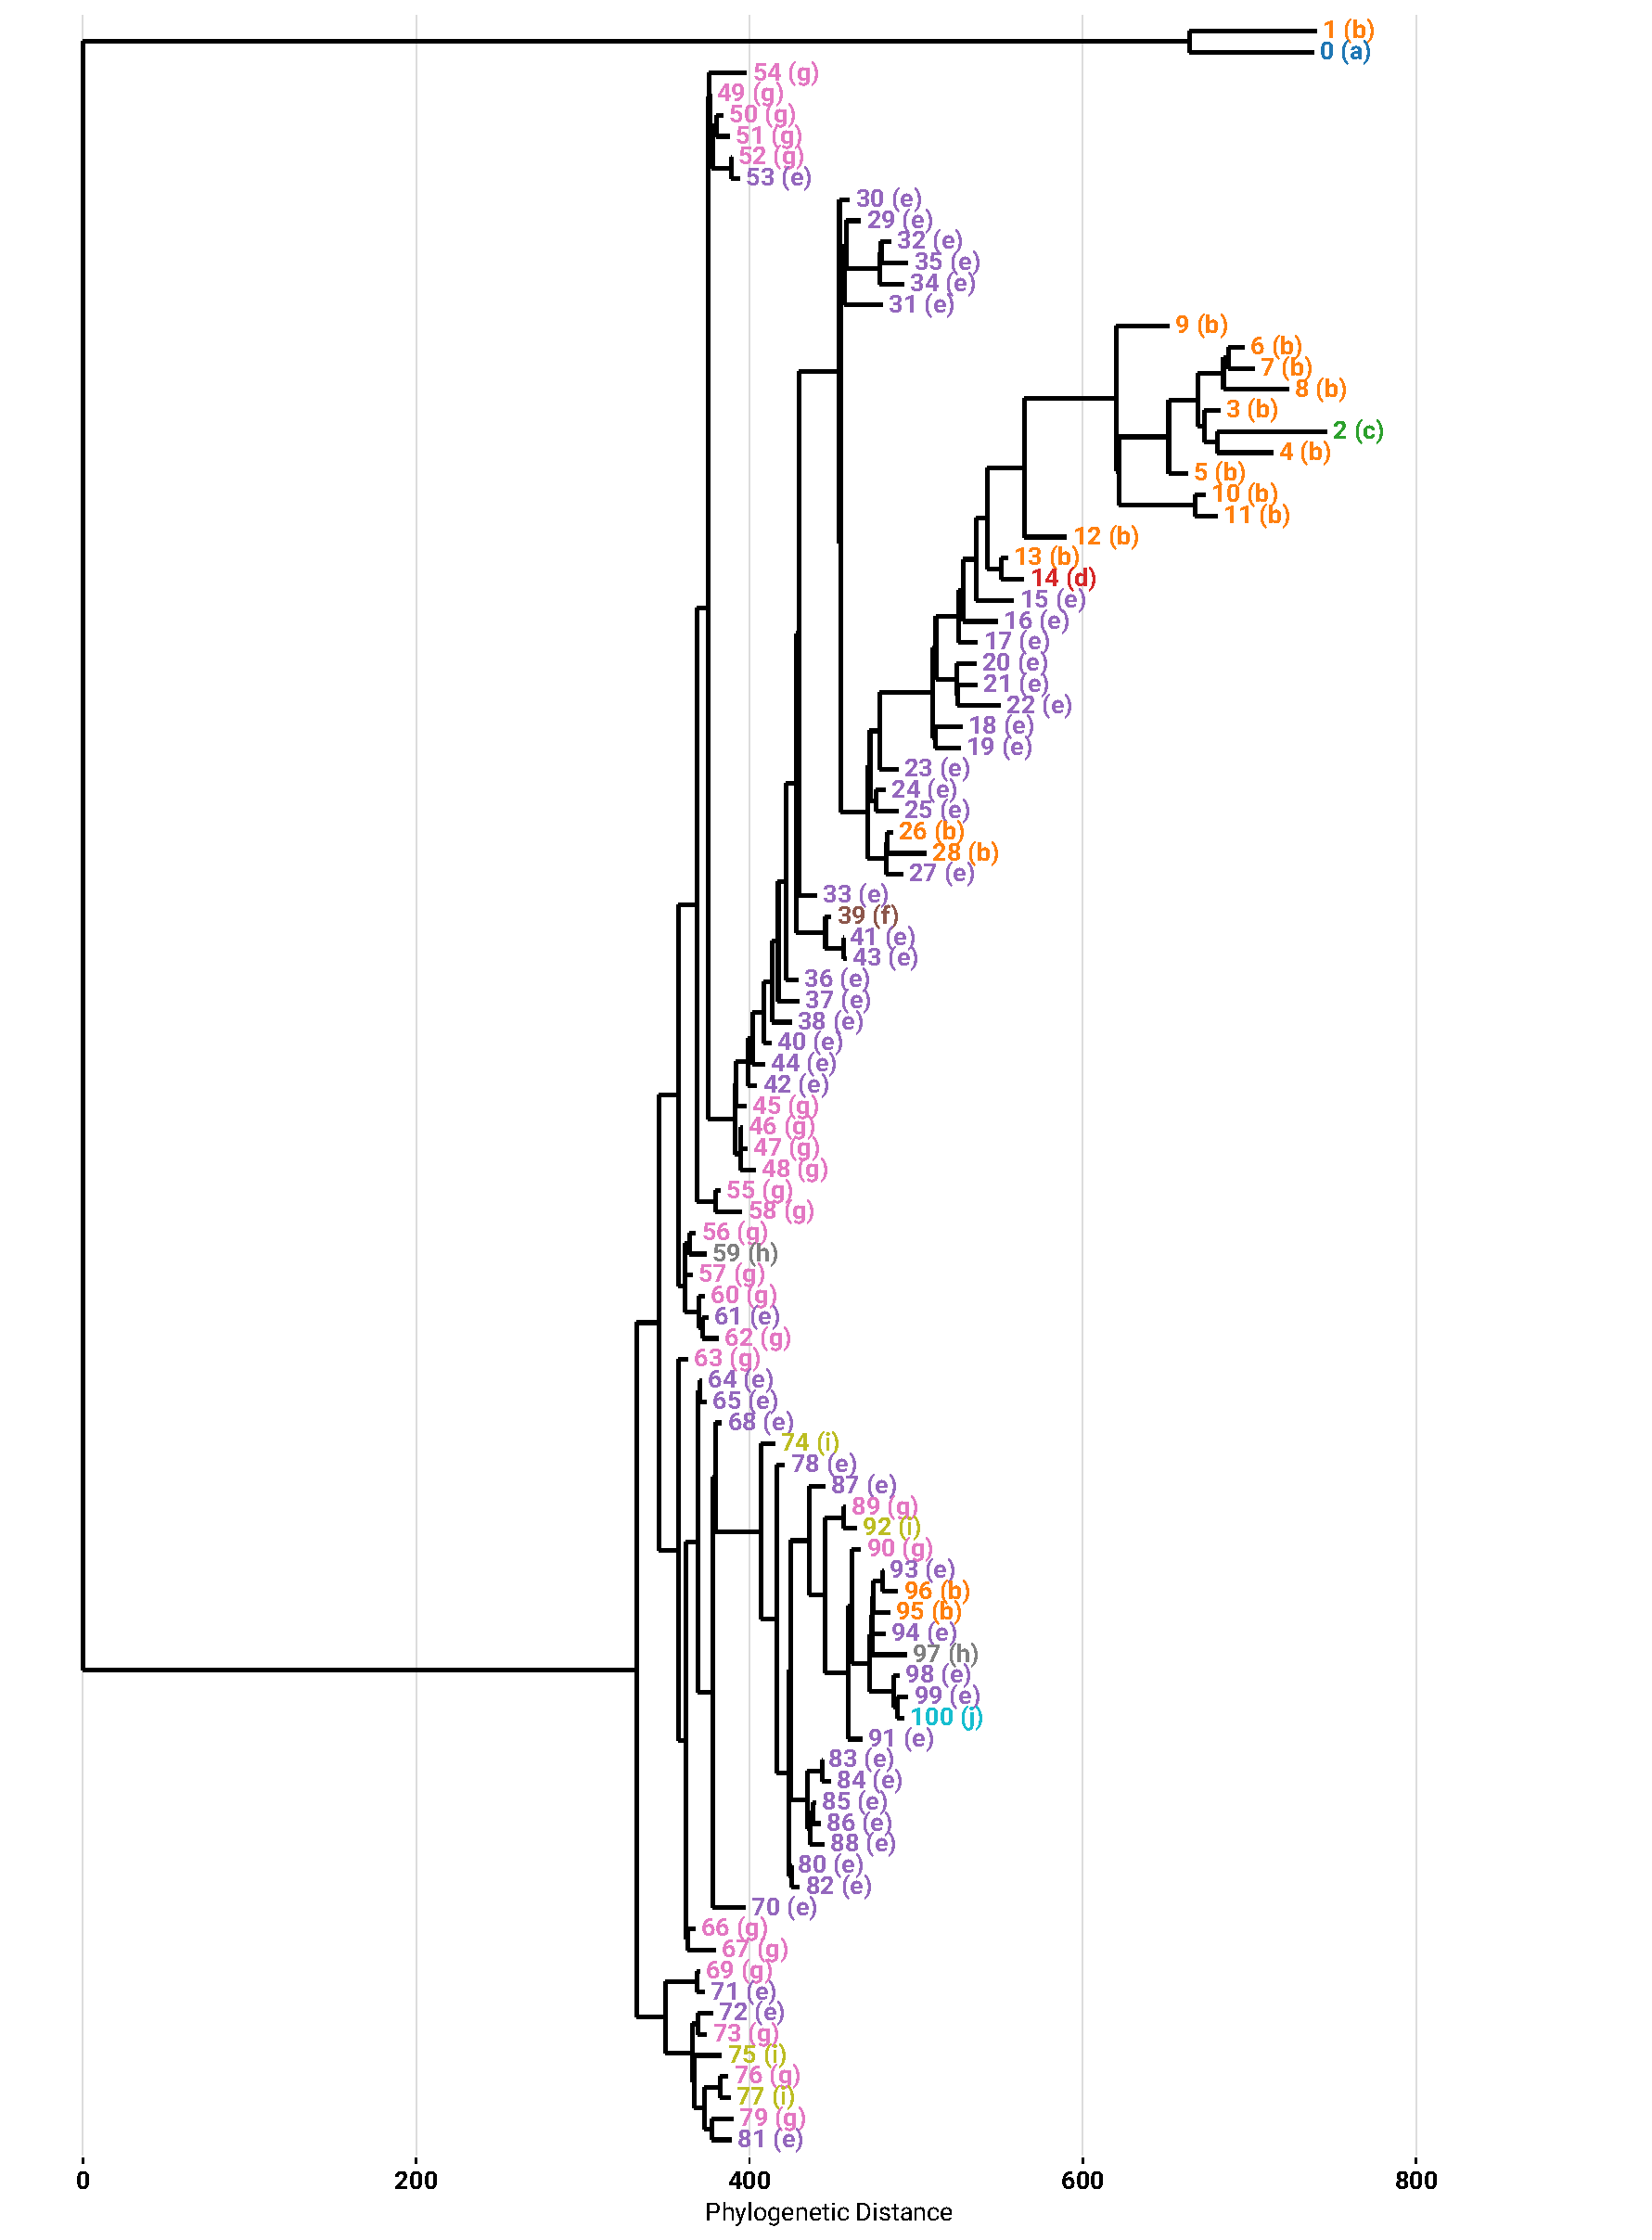
\includegraphics[width=0.8\linewidth]{{submodule/dishtiny_event_tag_phylogenetics/teeplots/ladderized_parsimony_tree_no_outliers/viz=draw+ext=}}

\caption{
\textbf{Estimated phylogeny of sampled focal strain representatives.}
\footnotesize
Phylogeny constructed using parsimony algorithm based on genome tag bitstring content \citep{cock2009biopython}.
Each leaf node corresponds to a sampled representative.
Representatives from stints 0 and 1, which share no common ancestry with representatives from other stints, are excluded.
Numbers refer to stint that each representative was sampled from.
Color coding and parentheticals of stint labels correspond to qualitative morph codes described in Table \ref{tab:morph_descriptions}.
}
\label{fig:phylo_parsimony_tree}
\end{figure*}


% https://github.com/mmore500/dishtiny_event_tag_phylogenetics/commit/ecc2ab8a580b125bea9f661e49cd4d7f34bfa1bb
In order to characterize the evolutionary history of the experiment in greater detail, we performed a parsimony-based phylogenetic reconstruction on the sampled representative specimens from each stint, shown in Figure \ref{fig:phylo_parsimony_tree}.
We used genomes' fixed-length blocks of 35 64-bit tags that mediate environmental interactions as the basis for this reconstruction.
These tag blocks underwent bitwise mutation over the course of the experiment.%
\footnote{
In future experiments, we plan to incorporate new methodology for ``hereditary stratigraph'' genome annotations expressly designed to facilitate phylogenetic reconstruction \dissertationelse{(Chapter \ref{ch:distributed-phylogeny})}{\citep{moreno2022hereditary}}.
}
Supplementary Figure \ref{fig:phylo_distance_matrix_heatmap} shows Hamming distance between all pairs of tag blocks.
We additionally tried several other tree inference methods, discussed in supplementary material; however, these yielded lower-quality reconstructions.

Although the phylogeny of stint representatives includes many instances that do not constitute a strict sequential lineage (i.e., each stint's representative descending directly from the preceding stint's representative), we did not observe evidence of long-term coexistence of clades over more than ten stints.

\subsection{Qualitative Morphological Categorizations}

% \pragmaonce

% adapted from https://www.overleaf.com/learn/latex/Commands
\providecommand{\dissertationelse}[2]{%
% adapted from https://tex.stackexchange.com/a/33577
\ifdefined\DISSERTATION
#1
\else
#2
\fi
}

% \pragmaonce

% adapted from https://www.overleaf.com/learn/latex/Commands
\providecommand{\dissertationexclude}[1]{%
% adapted from https://tex.stackexchange.com/a/33577
\ifdefined\DISSERTATION
\else
#1
\fi
}

% \pragmaonce

% adapted from https://www.overleaf.com/learn/latex/Commands
\providecommand{\dissertationonly}[1]{%
% adapted from https://tex.stackexchange.com/a/33577
\ifdefined\DISSERTATION%
#1%
\else%
\fi
}


\newcommand{\includesnapshot}[1] {%
\adjustbox{trim={0.05\width} {0.35\width} {0.05\width} {0.35\width},clip}%
    {\includegraphics[height=\dissertationexclude{0.3}\dissertationonly{0.25}\textheight]{#1}}
}
\newcommand{\morphtext}[1] {%
\color[HTML]{FFFFFF} \huge \raisebox{1.2em}{\textbf{#1}}%
}
\newcommand{\videolink}[1] {%
\raisebox{
\dissertationexclude{2.8em}
\dissertationonly{2.2em}
}{\begin{minipage}{\dissertationelse{2.4cm}{1.3 cm}} \dissertationelse{\fontsize{6}{7}\selectfont}{\tiny}\url{#1} \end{minipage}}
}
\newcommand{\descript}[1] {%
\raisebox{
  \dissertationexclude{2.8em}
  \dissertationonly{2.2em}
}{\begin{minipage}{\linewidth}\dissertationonly{\fontsize{8}{8}\selectfont} #1 \end{minipage}}
}


{
\catcode`\%=12
\begin{table*}
\begin{tabular}{cp{0.4\textwidth}ll}
\multicolumn{1}{l}{\textbf{ID}}               & \textbf{Morphology} & \textbf{Snapshot} & \textbf{Video} \\
\cellcolor[HTML]{4C72B0}{ \morphtext{a} } & \descript{Individual cells, no multicellular kin groups. Resource use is low---most cells simply hoard resource until their stockpile is beyond sufficient to reproduce. Only a handful of cells intermittently expend resource.} & \includesnapshot{\detokenize{snapshots/sanitized/a=kin-group-id+idx=0+proc=0+series=16005+stint=0+thread=0+update=28991+ext=.png}}             &  \videolink{https://hopth.ru/21/b=prq49+s=16005+t=0+v=video+w=specimen}          \\
\cellcolor[HTML]{DD8452}{\morphtext{b}} & \descript{Mostly individual cells, with some two-, three-, and four-cell groups evenly spread out. Resource usage occurs in short spurts in one or two adjacent cells. } & \includesnapshot{\detokenize{snapshots/sanitized/a=kin-group-id+idx=0+proc=0+series=16005+stint=1+thread=0+update=14271+ext=.png}}                 & \videolink{https://hopth.ru/21/b=prq49+s=16005+t=1+v=video+w=specimen}              \\
\cellcolor[HTML]{55A868}{\morphtext{c}} & \descript{Large multicellular groups dominate, consisting of hundreds of cells. Group growth is unchecked and continues until cells' resource stockpiles are entirely depleted by the excess group size penalty.} & \includesnapshot{\detokenize{snapshots/sanitized/a=kin-group-id+idx=0+proc=0+series=16005+stint=2+thread=0+update=17471+ext=.png}}                  & \videolink{https://hopth.ru/21/b=prq49+s=16005+t=2+v=video+w=specimen}             \\
\cellcolor[HTML]{C44E52}{\morphtext{d}} & \descript{Clear groups of 10 to 15 cells form. Cell proliferation appears somewhat more active at the periphery of groups compared to the interior.} & \includesnapshot{\detokenize{snapshots/sanitized/a=kin-group-id+idx=0+proc=0+series=16005+stint=14+thread=0+update=16959+ext=.png}}                  & \videolink{https://hopth.ru/21/b=prq49+s=16005+t=14+v=video+w=specimen}               \\
\cellcolor[HTML]{8172B3}{\morphtext{e}} & \descript{Groups are visibly elongated along the horizontal axis. After initial development, some gradual, irregular growth occurs along the vertical axis.} & \includesnapshot{\detokenize{snapshots/sanitized/a=kin-group-id+idx=0+proc=0+series=16005+stint=15+thread=0+update=16639+ext=.png}}                  & \videolink{https://hopth.ru/21/b=prq49+s=16005+t=15+v=video+w=specimen}              \\
\cellcolor[HTML]{937860}{\morphtext{f}} & \descript{Groups are horizontally elongated similarly to morphology $e$, but have a larger consistent vertical thickness of three or four cells.} & \includesnapshot{\detokenize{snapshots/sanitized/a=kin-group-id+idx=0+proc=0+series=16005+stint=39+thread=0+update=10303+ext=.png}}                  & \videolink{https://hopth.ru/21/b=prq49+s=16005+t=39+v=video+w=specimen}             \\
\cellcolor[HTML]{DA8BC3}{\morphtext{g}} & \descript{Initial group growth is almost entirely horizontal, with groups usually taking up only one row of cells. However, after an apparent timing cue groups perform a brief bout of aggressive vertical growth.} & \includesnapshot{\detokenize{snapshots/sanitized/a=kin-group-id+idx=0+proc=0+series=16005+stint=45+thread=0+update=12991+ext=.png}}                  & \videolink{https://hopth.ru/21/b=prq49+s=16005+t=45+v=video+w=specimen}              \\
\cellcolor[HTML]{8C8C8C}{\morphtext{h}} & \descript{Groups grow horizontally and then proliferate vertically on a timing cue like morph $e$. However, after that timing cue cell proliferation is incessant with almost no resource retention.} & \includesnapshot{\detokenize{snapshots/sanitized/a=kin-group-id+idx=0+proc=0+series=16005+stint=59+thread=0+update=11839+ext=.png}}                  & \videolink{https://hopth.ru/21/b=prq49+s=16005+t=59+v=video+w=specimen}              \\
\cellcolor[HTML]{CCB974}{\morphtext{i}} & \descript{Irregular groups of mostly less than ten cells. Incessant proliferation with almost no resource retention leads to rapid group turnover.} & \includesnapshot{\detokenize{snapshots/sanitized/a=kin-group-id+idx=0+proc=0+series=16005+stint=74+thread=0+update=12991+ext=.png}}                  & \videolink{https://hopth.ru/21/b=prq49+s=16005+t=74+v=video+w=specimen}              \\
\cellcolor[HTML]{64B5CD}{\morphtext{j}} & \descript{
Groups grow horizontally and then proliferate vertically on a timing cue like morph $e$. However, several viable horizontal-bar offspring groups form before forced fragmentation.} & \includesnapshot{\detokenize{snapshots/sanitized/a=kin-group-id+idx=0+proc=0+series=16005+stint=100+thread=0+update=8767+ext=.png}}                  & \videolink{https://hopth.ru/21/b=prq49+s=16005+t=100+v=video+w=specimen}
\end{tabular}

\caption{
\textbf{Qualitative morph phenotype categorizations.}
\footnotesize
Color coding of morph IDs has no significance beyond guiding the eye in scatter plots where points are labeled by morph.
Snapshot visualizes spatial layout of kin groups on toroidal grid at a fixed point in time.
Each cell corresponds to a small square tile.
Color hue denotes, and black borders divide, outermost kin groups; color saturation denotes, and white borders divide, innermost kin groups.
}
\label{tab:morph_descriptions}

\end{table*}
}


We performed a qualitative survey of the evolved life histories along the evolutionary timeline by reviewing video animations of the representative specimen from each stint in monoculture.

Table \ref{tab:morph_descriptions} summarizes the ten morphological categories we grouped specimens into.
In brief, specimens from early stints largely grew as unicellular or small multicellular groups (morphs $a$, $b$).
Then, the specimen from stint 14 grew as larger, symmetrical groups (morph $d$).
At stint 15, a distinct, asymmetrical horizontal bar morphology evolved (morph $e$).
%todo structure above is confusing
% Consistently left/right, indicating that somehow broke symmetrical of the simulation.
At stint 45, a delayed secondary spurt of group growth in the vertical direction arose (morph $g$).
This morphology was sampled frequently until stint 60, when morph $e$ began to be sampled primarily again.
However, morph $g$ was observed as late as stint 90.

Phylogenetic analysis (Figure \ref{fig:phylo_parsimony_tree}) indicates that observations of morph $e$ at stint 53 and onward are instances of secondary loss rather than retention of trait $e$ by a separate lineage coexisting with the lineage expressing morph $g$.
Three separate reversion events from morph $g$ to morph $e$ appear likely.
Interestingly, morph $g$ individuals at stints 89 and 90 appear to represent subsequent trait re-gain after reversion from morph $g$ to morph $e$.

Table \ref{tab:morph_descriptions} provides more detailed descriptions of each qualitative morph category, as well as a video and still image example of each.

Supplementary Table \ref{tab:morph_by_stint} provides morph categorization for each stint as well as links to view the stint's specimen in a video or in-browser web simulation.

% \subsection{Multicellular Phenotypic Traits}

% In order for a transition in individuality, cells have to diminish their own immediate reproductive interests in order to prioritize the interests of the collective.
% In previous work with an earlier version of the system, we've seen multicellular traits evolve such as (blah from abstract) %todo
% \citep{moreno2021exploring}.

% The formation of kin group morphologies in this system does not necessarily imply a transition in individuality.
% It is necessary to test to see if cells within groups are meaningfully cooperating.

% Because cell reproduction is necessarily adversarial in this system, we can test to see whether cells preferentially target or spare their group members.
% A conflict ratio of less than 1 implies that cells preferentially spare their members.
% We observed a  0.5 most of the time.

% Supplementary Figure \ref{fig:conflict:exactly_one} shows the  . %todo
% Supplementary Figure \ref{fig:conflict:at_least_one}
% Supplementary Figure \ref{fig:conflict:exactly_two}.
% However, could be an artifact of cell-offspring cooperation.

% Interestingly, this strain appears to be using ``Is Child Cell Of,'' ``Is Parent Cell Of,'' ``Is Child Group Of,'' and the raw kin group ID of neighbors (but not the raw kin group ID of self).

% %todo change wording, not sure what you're hoping to say with first phrase
% To more conclusively, in future work we plan to look at the reproductive output at the interior of multicellular groups to see if these cells diminish their own reproductive output and to control for cellular relatedness when calculating this element of group cooperation.

% We analyzed other traits characteristic of multicellularity, as well.

% We did not see widespread resource sharing over the evolutionary history.
% Only tiny fractions of cells, less than 1\%, appeared to share tiny amounts of the resource, less than 1\% of the resource required to reproduce per update (Supplementary Figures \ref{fig:resource_sharing:fraction_sharing_monoculture} and \ref{fig:resource_sharing:sharing_amount_monoculture}).
% However, in ten strains sampled along the evolutionary lineage, context-dependent resource-sending behavior contributed to fitness (Supplementary Figure \ref{fig:writable_perturbation}).
% Interestingly, another strain present in the population that was not the subject of analysis appeared to evolve widespread, higher-throughput resource sharing after stint 60 (Supplementary Figures \ref{fig:resource_sharing:fraction_sharing_evolve} and \ref{fig:resource_sharing:sharing_amount_evolve}).

% We observed widespread apoptosis over the evolutionary history.
% As shown in Supplementary Figure \ref{fig:apoptosis:apoptosis_stint}, in most monocultured representative strains, between 10 and 30\% of cell deaths were due to apoptosis.
% However, it is not clear if this apoptosis returned a fitness benefit.
% No context-dependent apoptosis behavior contributed to fitness for any sampled strain over the evolutionary history (Supplementary Figure \ref{fig:writable_perturbation}).
% It is unclear whether context-independent apoptosis might have a fitness benefit.

% The behavior seems like cells from within a group don't explicitly recognize one another according to group membership. However, they do recognize their cell parent/child and arrange themselves in a somewhat linear fashion that minimizes the potential for conflict between cells.
% Overall, there are elements of cooperation but is unclear to what extent this particular strain constitutes a proper fraternal transition in individuality.

\subsection{Fitness}

% \begin{figure}

\begin{subfigure}{0.5\textwidth}

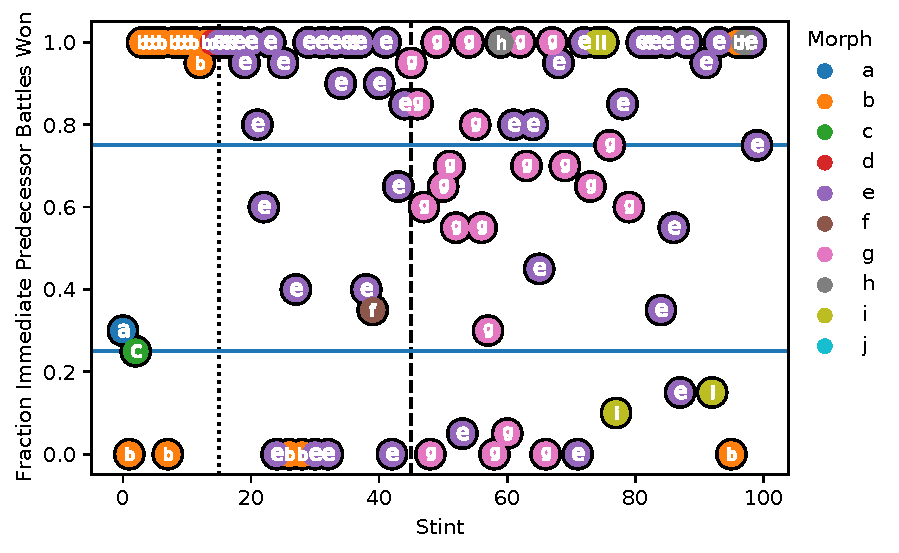
\includegraphics[width=\linewidth]{{plots/fitness/bucket=prq49+cat=morph+endeavor=16+transform=filter-Series-16005+viz=letterscatter-vline-binomialh0+x=stint+y=fraction-immediate-predecessor-battles-won+ext=}}

\caption{
Fraction of 20 independent competitions that were won against immediate predecessor population.
Blue horiziontal lines represent significance level $p < 0.05$ for binomial null hypothesis.
Neutral outcomes fall inside the blue bars, significant fitness increases fall above them, and significant fitness decreases fall below them.
}
\label{fig:fitness:fitness_neutrality}

\end{subfigure}%

\begin{subfigure}{0.5\textwidth}

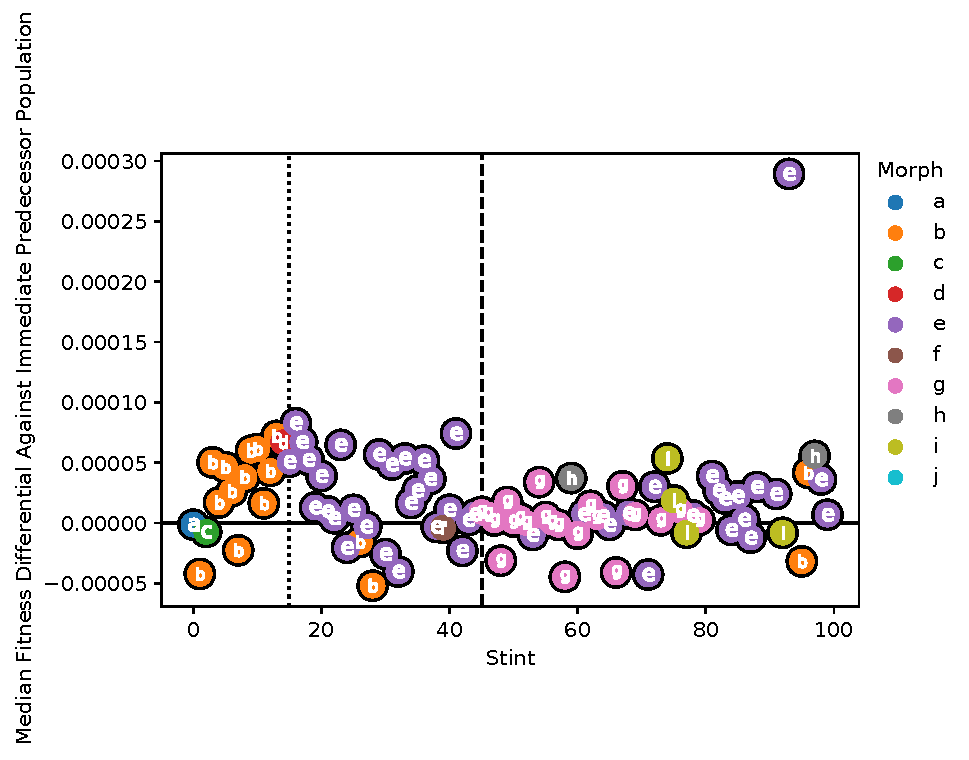
\includegraphics[width=\linewidth]{{plots/fitness/bucket=prq49+cat=morph+endeavor=16+transform=filter-Series-16005+viz=letterscatter-vline-hline+x=stint+y=median-fitness-differential-against-immediate-predecessor-population+ext=}}

\caption{Magnitude of fitness differential against immediately-preceding stint population.
Positive fitness differential indicates greater fitness compared to predecessor.
Solid horizontal line indicates neutral fitness differential.
}
\label{fig:fitness:fitness_magnitude}

\end{subfigure}%

\begin{subfigure}{0.5\textwidth}

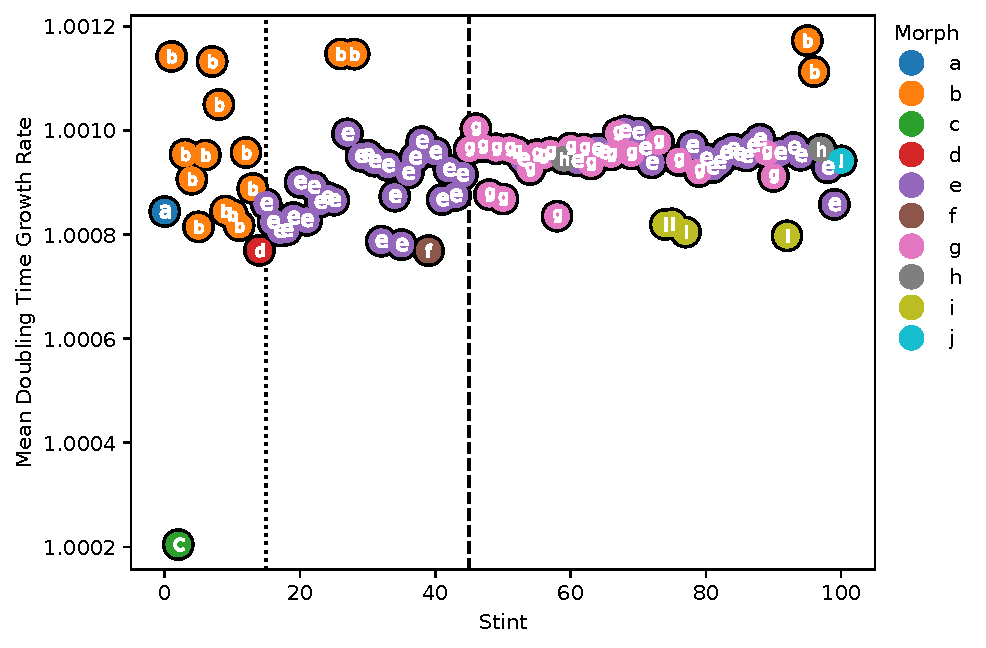
\includegraphics[width=\linewidth]{{plots/fitness/bucket=prq49+cat=morph+endeavor=16+transform=filter-Series-16005+viz=letterscatter-vline+x=stint+y=mean-doubling-time-growth-rate+ext=}}

\caption{Growth rate estimated from doubling time experiments, measuring time for a monoculture to grow from 0.25 maximum population size to 0.5 maximum population size.}
\label{fig:fitness:doubling_time}

\end{subfigure}%


\caption{ Fitness assays.
Color coding and letters correspond to qualitative morph codes described in Table \ref{tab:morph_descriptions}.
Dotted vertical line denotes emergence of morph $e$.
Dashed vertical line denotes emergence of morph $g$. }
\label{fig:fitness}

\end{figure}

\begin{figure*}

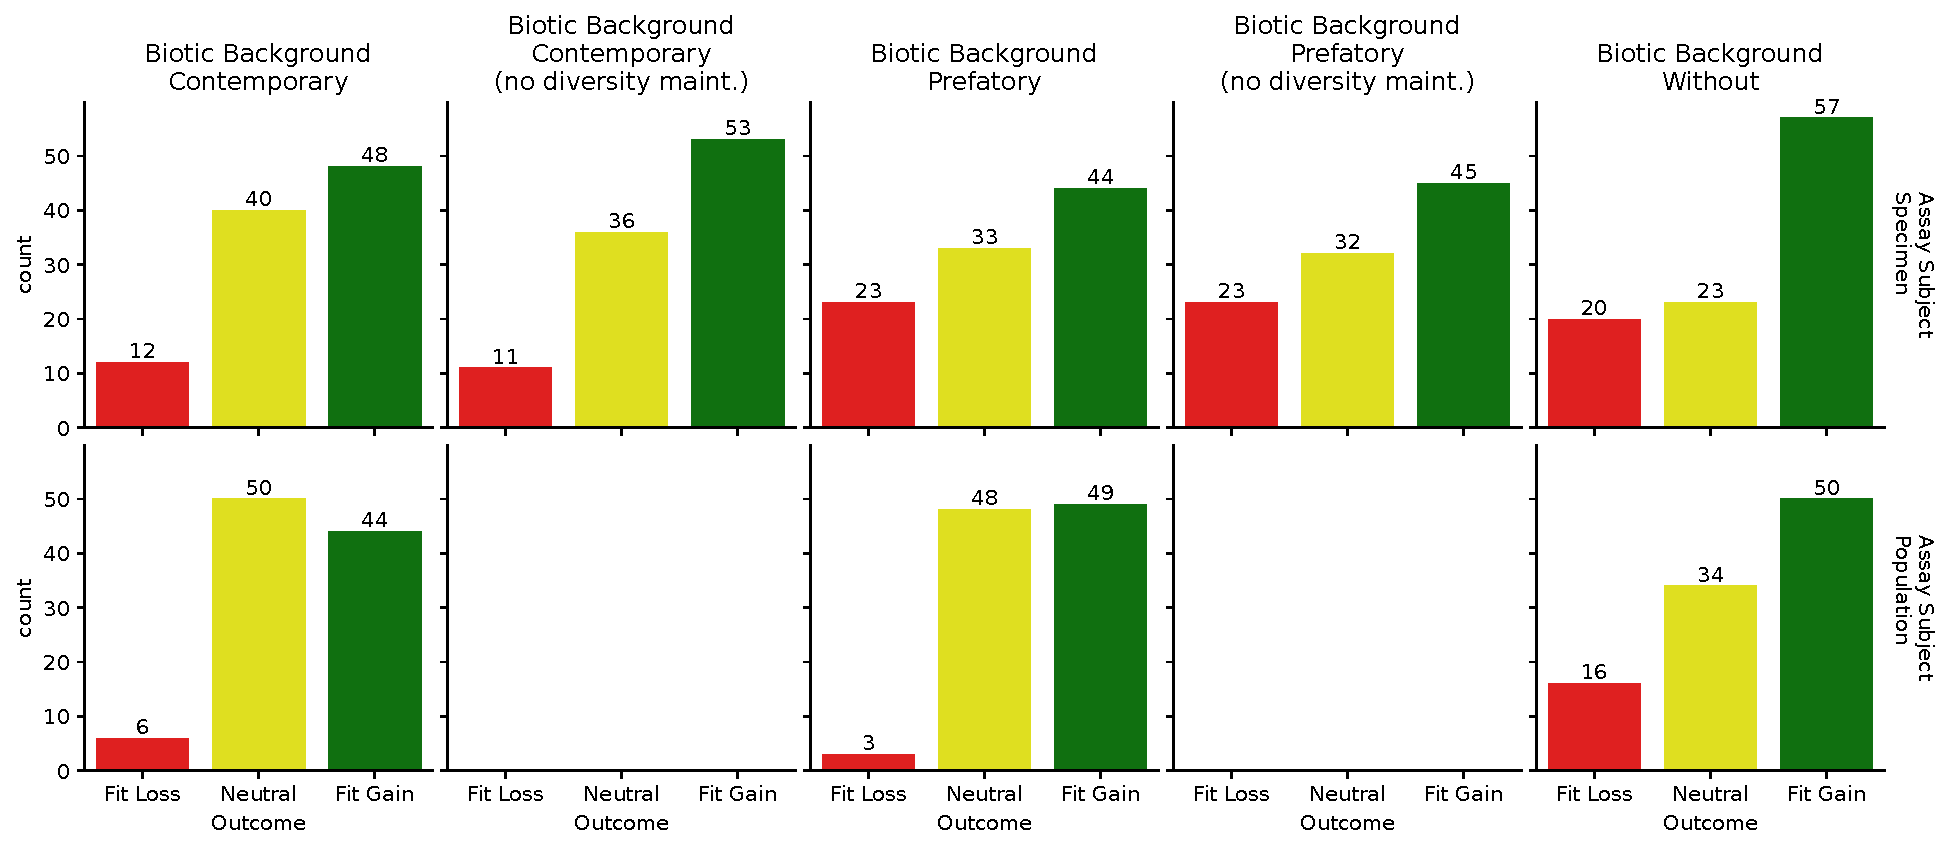
\includegraphics[width=\linewidth]{{submodule/dishtiny/binder/bucket=prq49/a=adaptation_assays+endeavor=16/teeplots/col=biotic-background+kind=count+row=assay-subject+viz=barlabel-catplot+x=outcome+ext=}}

\caption{
TODO
}
\label{fig:outcome_count_distns}
\end{figure*}


Of the 100 competition assays performed, 57 indicated significant fitness gain, 23 were neutral, and 20 indicated significant fitness loss (shown in upper right of Figure \ref{fig:outcome_count_distns}, at the intersection of the ``Biotic Background, Without'' column and ``Assay Subject, Specimen'' row.)

We were surprised by the frequency of deleterious outcomes, leading us to perform a second set of experiments to investigate whether these outcomes could be explained as sampling of ``dud'' representatives.
In these competition assays, we competed the entire focal strain population against the focal strain population from the preceding stint.
However, we observed a similar result: 50 assays indicated significant fitness gain, 34 were neutral, and 16 indicated significant fitness loss (shown in lower right of Figure \ref{fig:outcome_count_distns}, at the intersection of the ``Biotic Background, Without'' column and ``Assay Subject, Population'' row.)

\begin{figure*}
\centering
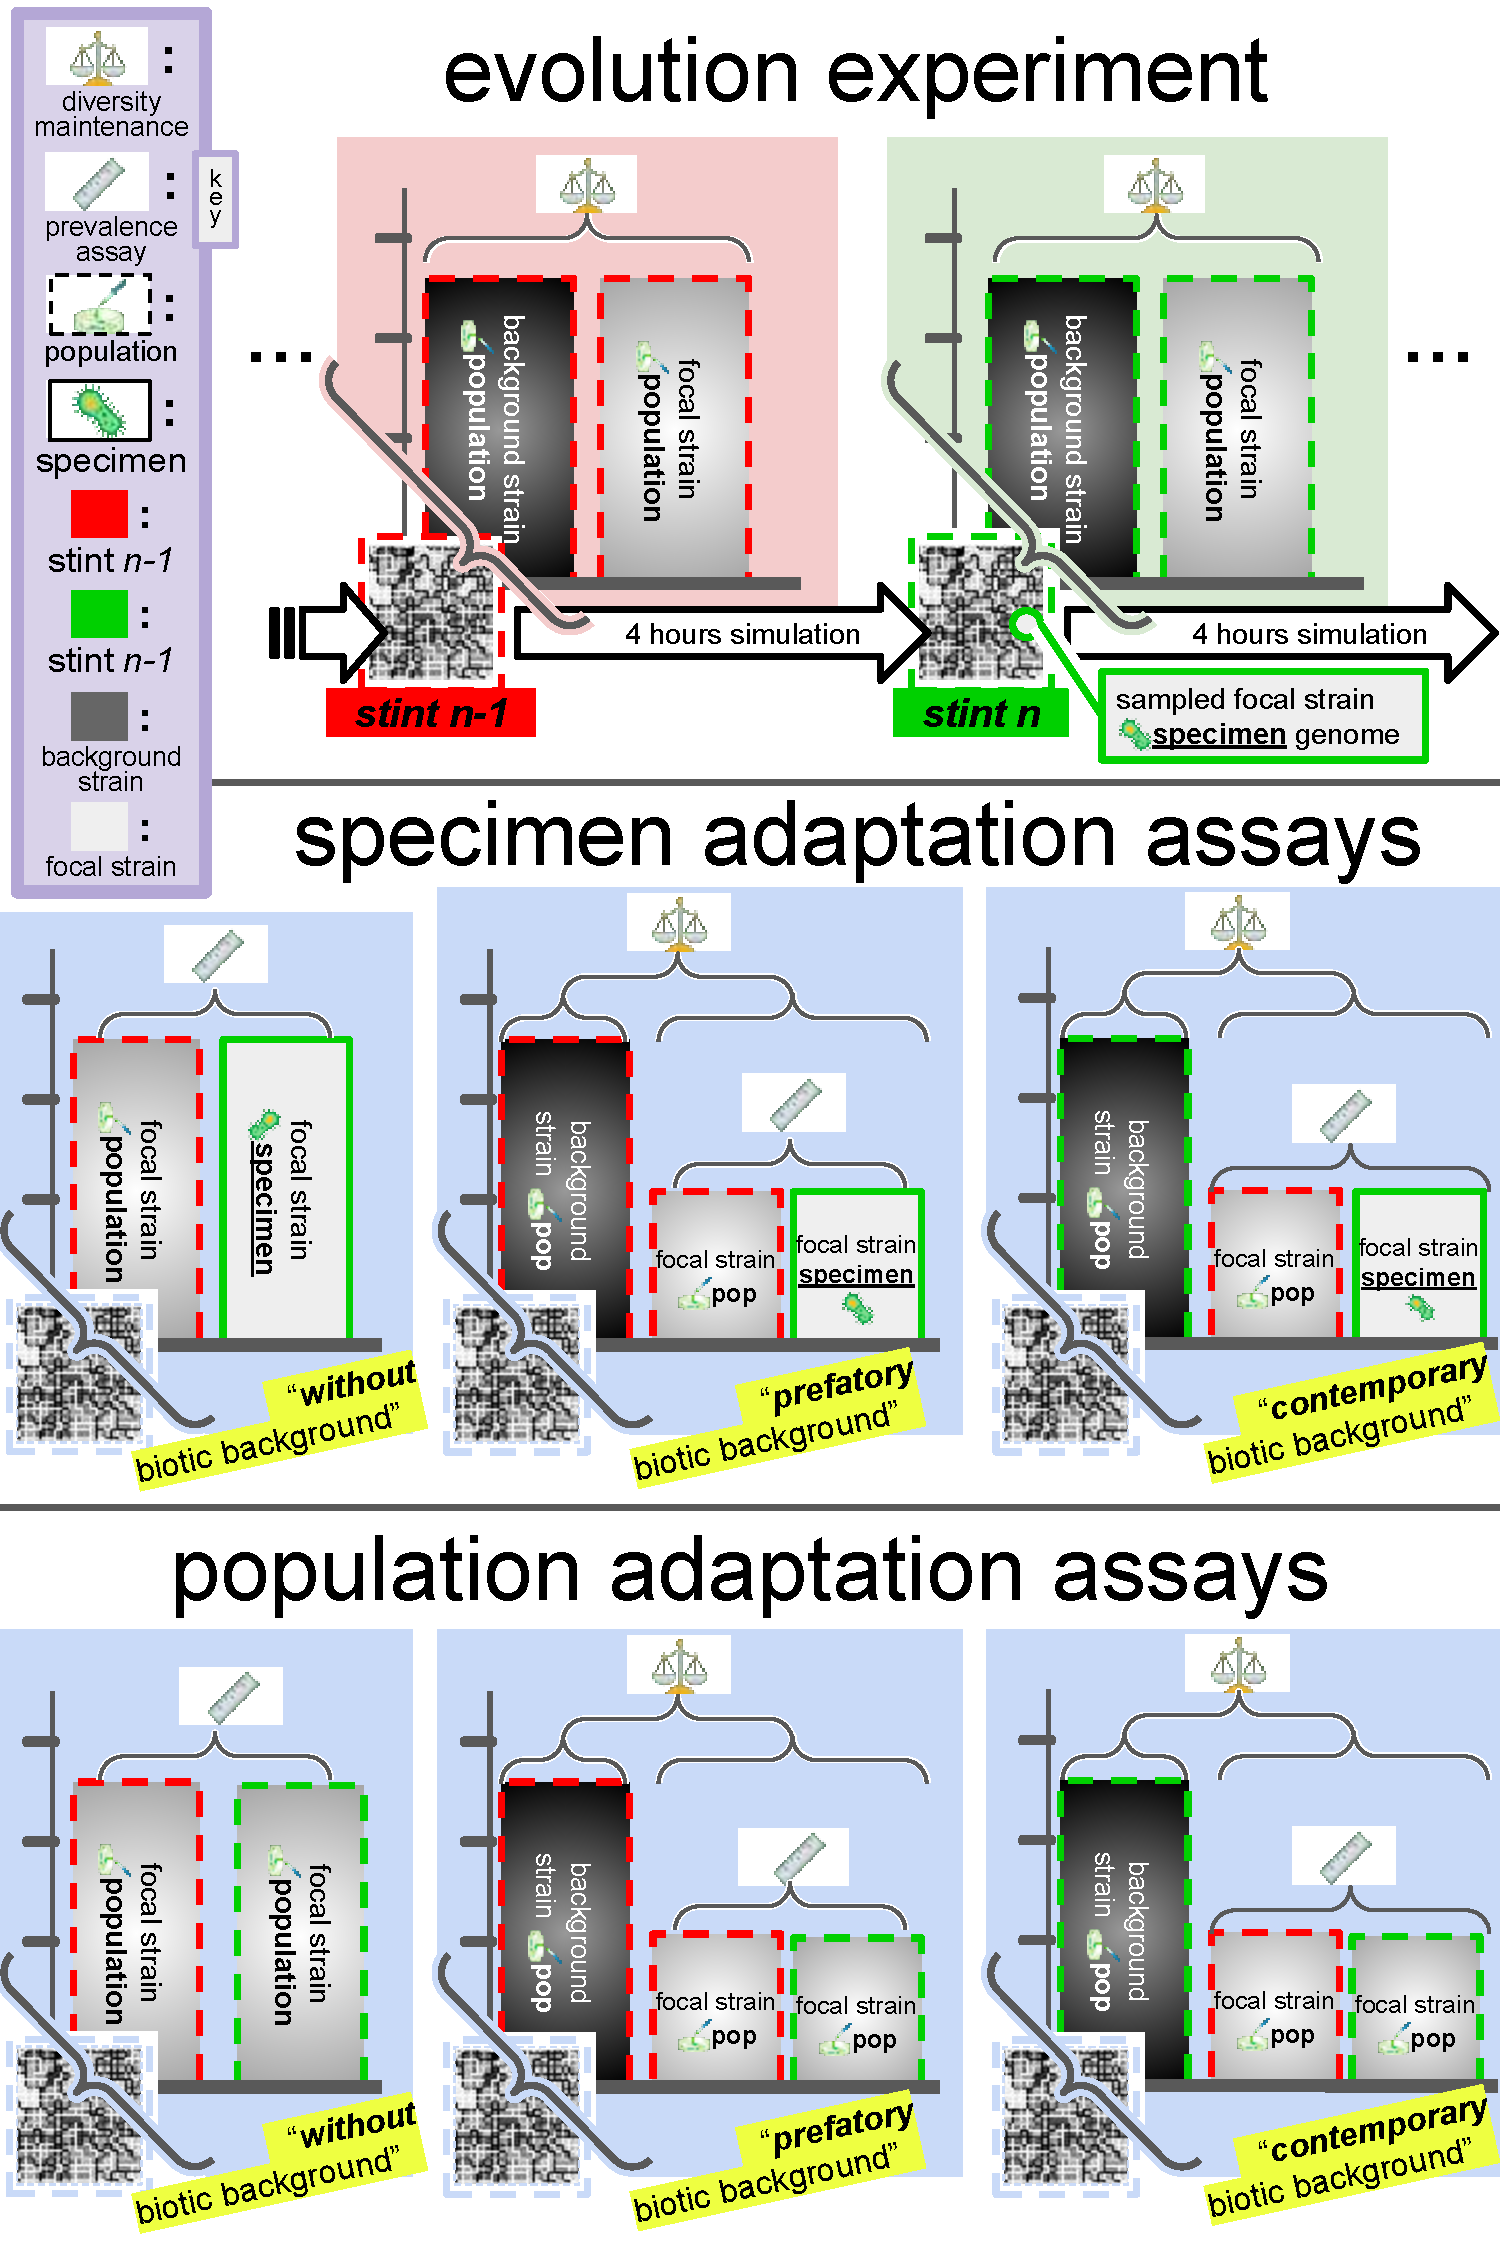
\includegraphics[width=0.5\linewidth]{{img/adaptation-assay-cartoon}}

\caption{
Detail of adaptation assay design.
Top panel shows progress of original evolutionary experiment over one stint.
A diversity maintenance procedure was used to ensure long-term coexistence of a least two strains over the course of the experiment by penalizing any strain that occupied more than half of thread-local population space.
A ``focal strain'' was arbitrarily chosen for study; we refer to the other strain as the ``background strain.''
Adaptation assays in lower panels measure fitness change over the course of that stint through against the population from the preceding stint.
The middle panel shows measurement of adaptation of the representative specimen that was sampled for analysis at each stint.
The bottom panel shows measurement of the adaptation of the entire focal strain population at each stint.
Competitors were mixed in even proportion into the environment.
Bar heights represent initial relative proportions of assay participants at the beginning of the competition.
Adaptation was measured by measuring change in population composition over a 10 minute competition window.
We call this measurement of population composition change a ``prevalence assay''.
Competition experiments were performed absent the background strain, with the background strain population from the preceding stint, or with the background strain population from the current stint --- shown separately in each panel.
}
\label{fig:adaptation_assay_cartoon}
\end{figure*}


Next, we investigated whether the presence of the background strain as a ``biotic background'' influenced fitness.
We repeated the two experiments described above (specimen and population competition assays), but inserted the background strain as half of the initial well-mixed population.
In one assay setup, we used the background strain population from the current stint.
We refer to this as ``contemporary biotic background.''
In another, which we call ``prefatory biotic background,'' we used the background strain population from the previous stint.
We refer to the original competition assays absent the background strain as ``without biotic background.''
Figure \ref{fig:adaptation_assay_cartoon} summarizes these competition assay designs.

\begin{sidewaysfigure*}
\thisfloatpagestyle{mylandscape}%
\rotatesidewayslabel%
\centering

\begin{subfigure}[t]{0.32\textwidth}
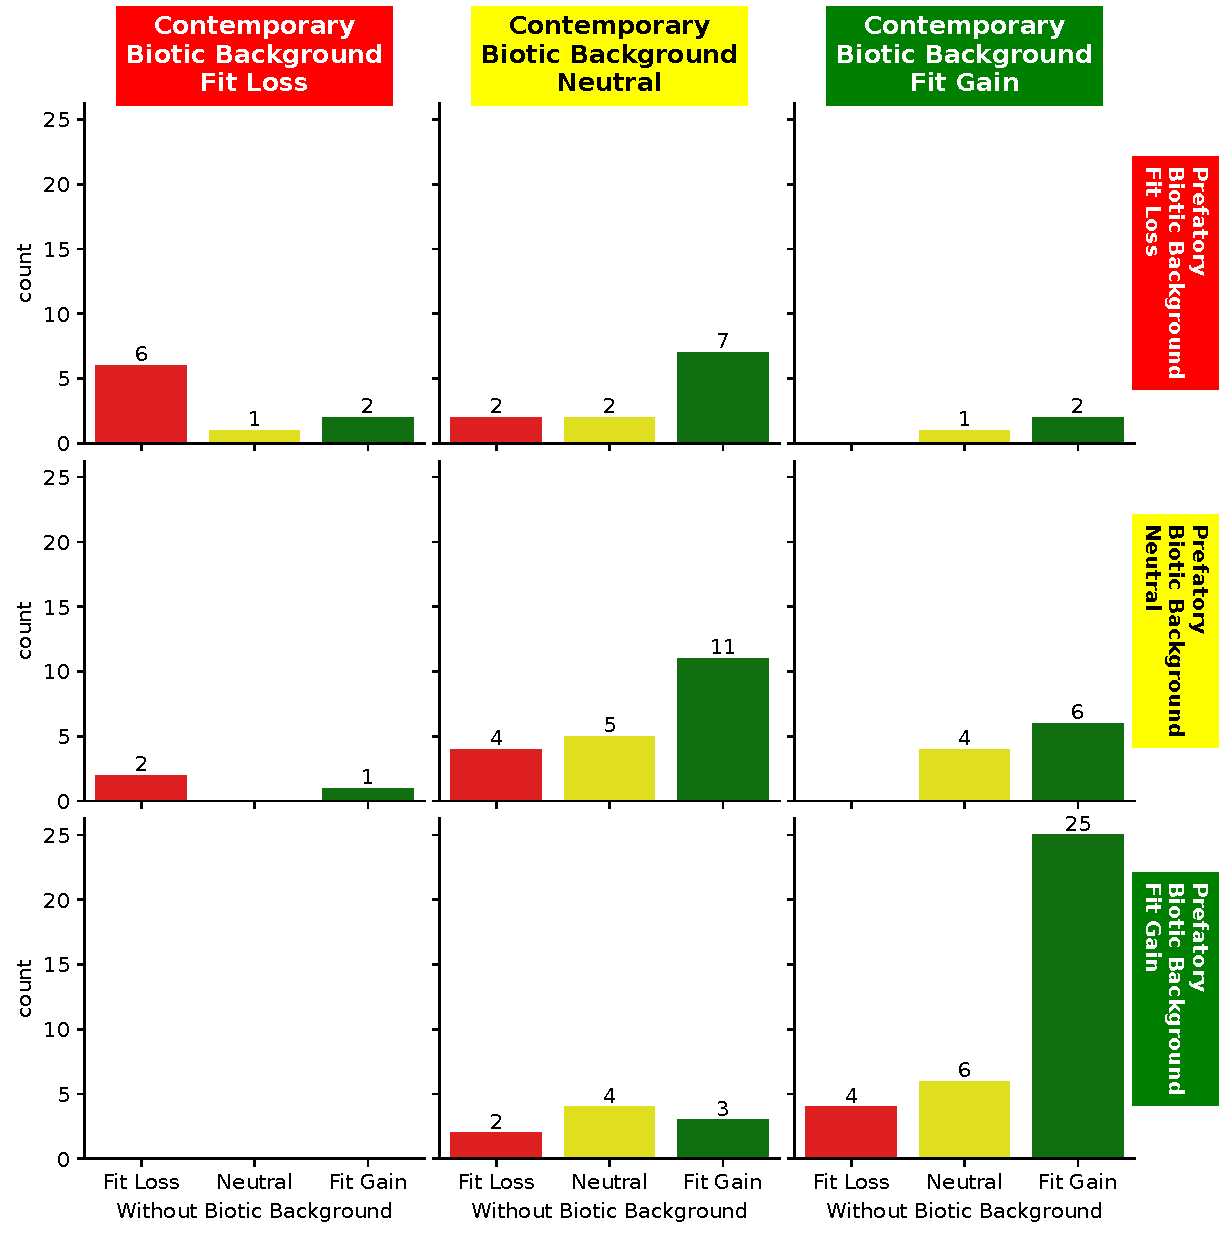
\includegraphics[width=\linewidth]{{submodule/dishtiny/binder/bucket=prq49/a=adaptation_assays+endeavor=16/teeplots/assay-subject=Specimen+col=contemporary-biotic-background+kind=count+row=prefatory-biotic-background+viz=barlabel-catplot+x=without-biotic-background+ext=}}
\caption{Joint distribution of adaptation assay on representative specimen from focal strain over biotic backgrounds, with diversity maintenance during competition.}
\label{fig:outcome_count_joint_distns:specimen_with_dm}
\end{subfigure}%
\hfill%
\begin{subfigure}[t]{0.32\textwidth}
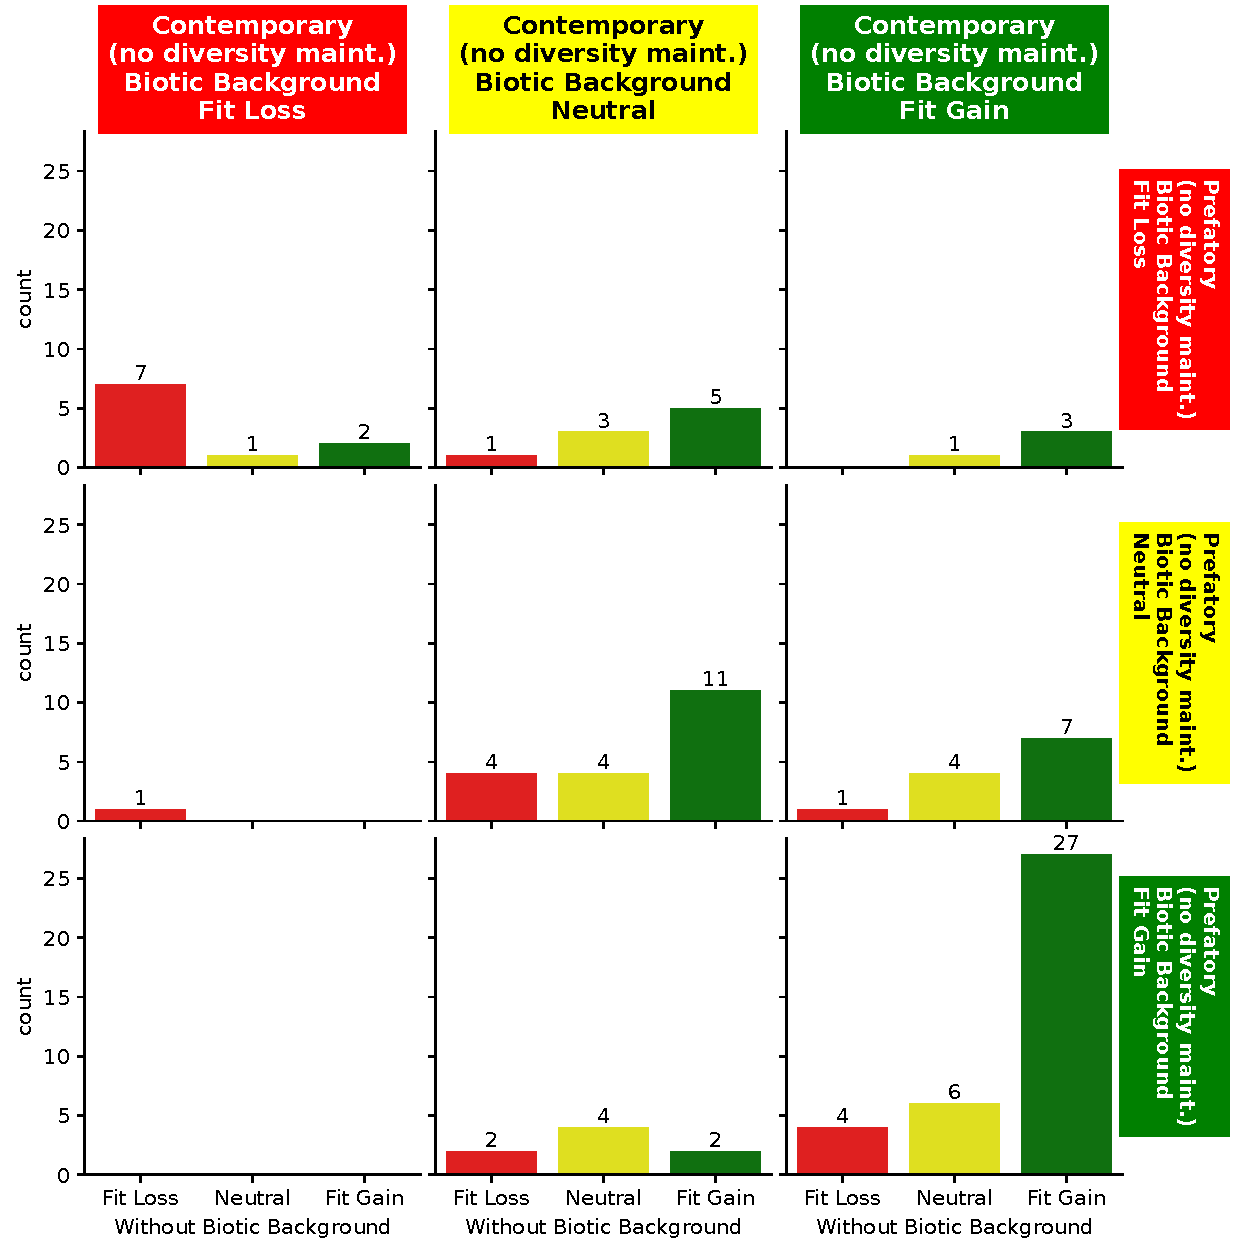
\includegraphics[width=\linewidth]{{submodule/dishtiny/binder/bucket=prq49/a=adaptation_assays+endeavor=16/teeplots/assay-subject=Specimen+col=contemporary-no-diversity-maint-biotic-background+kind=count+row=prefatory-no-diversity-maint-biotic-background+viz=barlabel-catplot+x=without-biotic-background+ext=}}
\caption{Joint distribution of adaptation assay on representative specimen from focal strain over biotic backgrounds, with diversity maintenance disabled during competition.}
\label{fig:outcome_count_joint_distns:specimen_no_dm}
\end{subfigure}%
\hfill%
\begin{subfigure}[t]{0.32\textwidth}
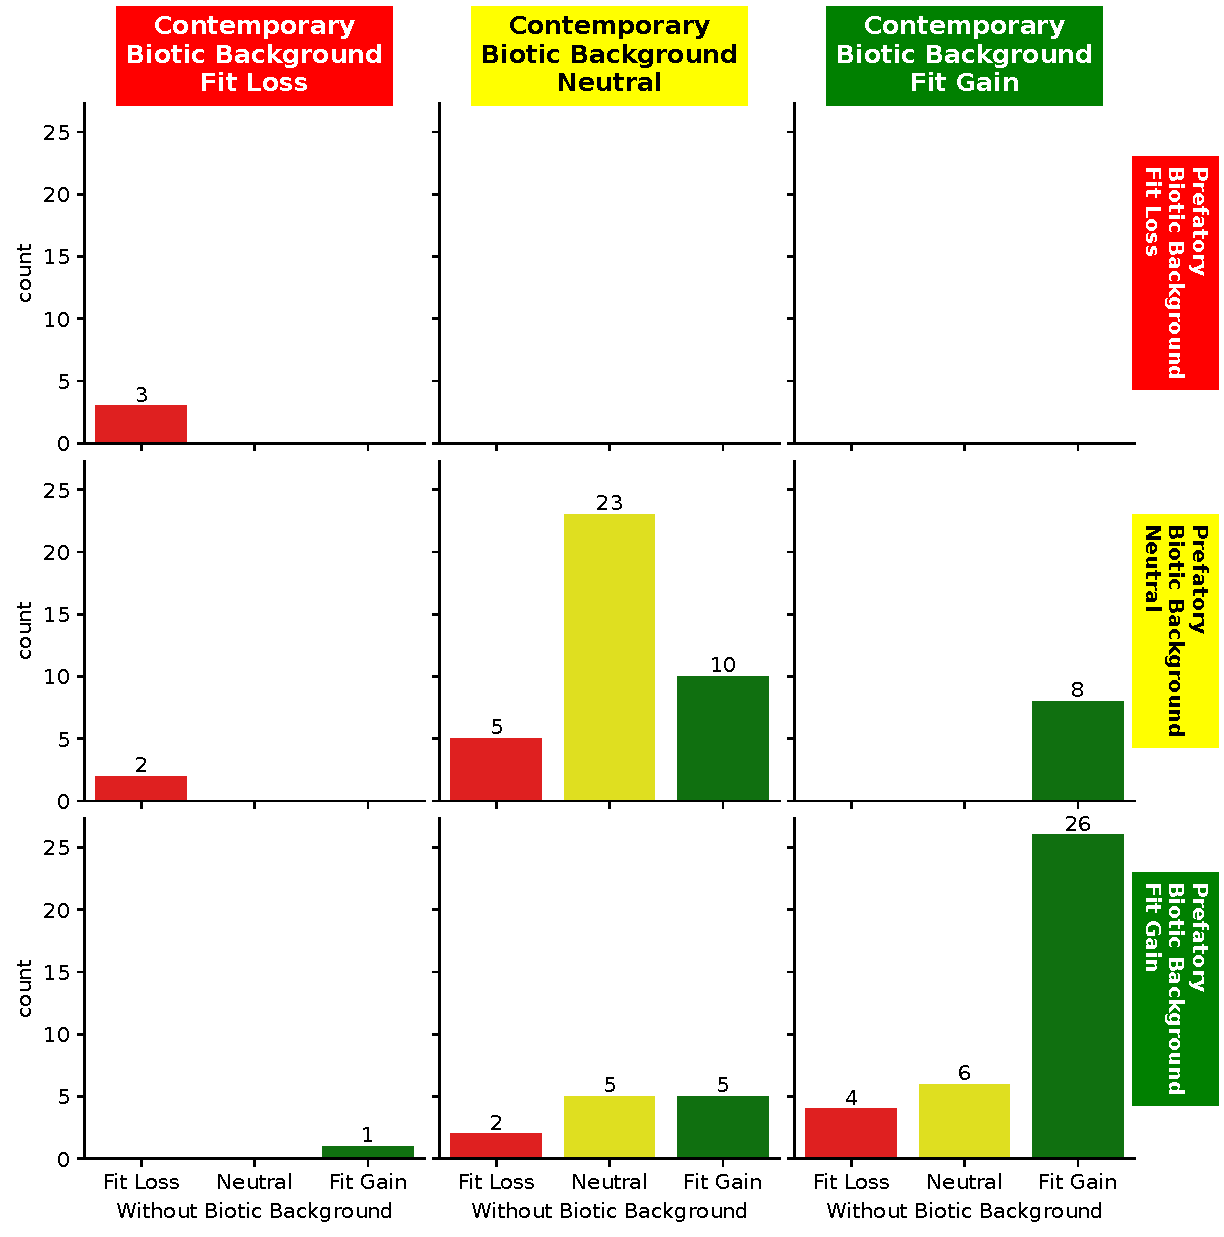
\includegraphics[width=\linewidth]{{submodule/dishtiny/binder/bucket=prq49/a=adaptation_assays+endeavor=16/teeplots/assay-subject=Population+col=contemporary-biotic-background+kind=count+row=prefatory-biotic-background+viz=barlabel-catplot+x=without-biotic-background+ext=}}
\caption{Joint distribution of adaptation assay on focal strain population over biotic backgrounds, with diversity maintenance during competition.}
\label{fig:outcome_count_joint_distns:population}
\end{subfigure}


\caption{
\textbf{Effect of biotic background on adaptation assay outcomes.}
\footnotesize
Joint distribution of adaptation assay outcomes across biotic backgrounds.
For each adaptation assay, three outcomes were possible: significant fitness gain, significant fitness loss, or no significant fitness change (``neutral'').
Significance cutoff $p < 0.005$ was used.
A fitness loss --- color-coded red --- corresponds to winning 2 or fewer competitions out of 20 against the preceding stint's focal strain population.
A fitness gain --- color-coded green --- corresponds to winning 18 or more competitions out of 20 against the preceding stint's focal strain population.
Neutral fitness outcomes are color-coded yellow.
Outcome counts are accumulated over experiments from stint 1 through stint 100.
Counts in each subfigure therefore sum to 100.
Column position in facet grid indicates outcome with contemporary biotic background, row position indicates outcome with prefatory biotic background, and bar color and $x$ position indicates outcome without biotic background.
See Figure \ref{fig:adaptation_assay_cartoon} for explanation of competition biotic backgrounds.
See Figure \ref{fig:with_vs_without_diversity_maintenance} for detail on joint distribution of outcomes with and without diversity maintenance, which were mostly identical.
}
\label{fig:outcome_count_joint_distns}
\end{sidewaysfigure*}


After incorporating the background strain into our measure of fitness, we detected fewer whole-population deleterious outcomes --- only six under contemporary biotic background conditions and only three under prefatory biotic background conditions (Figure \ref{fig:outcome_count_distns}).
To determine whether the presence of the background strain caused the overall reduction in whole-population deleterious outcomes, we performed control competitions under biotic background conditions, but with the focal strain population substituted for the background strain population (Supplementary Figure \ref{fig:baseline_adaptation_control}).
Under these conditions, nine of the stints where whole-population deleterious outcomes had been detected came up neutral;
one, surprisingly, tested significantly adaptive (Supplementary Figure \ref{fig:baseline_fitness_gain_or_loss}).
Dose-dependent fitness effects and/or reduced experimental sensitivity of the biotic background assay appear to play at least a partial role in explaining the reduction of detected whole-population deleterious outcomes.
However, 10 stints still tested significantly deleterious with the control focal strain biotic background in addition to without biotic background.

Four stints do provide strong, direct evidence of a selective effect by the background strain: four whole-population outcomes that were deleterious without their biotic background were actually significantly advantageous in the presence of both the prefatory and contemporary background strain populations (Figure \ref{fig:outcome_count_joint_distns:population}).
All four of these stints exhibited whole-population deleterious outcomes under the control focal strain biotic background, indicating that the observed fitness sign change was specifically due to the presence of the background strain (Supplementary Figure \ref{fig:baseline_fitness_gain_or_loss}).

Additionally, we detected two deleterious outcomes without biotic background as significantly adaptive under the prefatory biotic background but as neutral under contemporary biotic background (Figure \ref{fig:outcome_count_joint_distns:population}).
Control focal strain biotic background experiments again suggest that the background strain, specifically, is responsible for this effect (Supplementary Figure \ref{fig:baseline_fitness_gain_or_loss}).

% A further five outcomes were detected as significantly deleterious without biotic background but were not detected as significantly adaptive or deleterious (i.e., neutral) in the presence of both background strain populations (Figure \ref{fig:outcome_count_joint_distns:population}).
We also found one whole-population outcome that was significantly advantageous without biotic background and in the presence of the prefatory background strain population but significantly deleterious in the presence of the contemporary background strain, possibly suggesting an ``arms race''-like evolutionary innovation on the part of the background strain over that stint (Figure \ref{fig:outcome_count_joint_distns:population}).

Nonetheless, we still saw three whole-population outcomes that were significantly deleterious under all three conditions (Figure \ref{fig:outcome_count_joint_distns:population}).
These whole-population outcomes were also deleterious under the control focal strain biotic background experiments (Supplementary Figure \ref{fig:baseline_fitness_gain_or_loss}).
Muller's ratchet \citep{andersson1996muller} or maladaptation due to environmental change \citep{brady2019causes} may offer possible explanations, but a definitive answer will require further study.

We also performed fitness assays on individual sampled specimens with both biotic backgrounds.
Out of 100 stints tested, we observed 20 significantly deleterious outcomes without biotic background, 23 significantly deleterious outcomes under prefatory biotic background, and 12 significantly deleterious outcomes under contemporary biotic background (Figure \ref{fig:outcome_count_distns}).
Unlike the whole-population deleterious outcomes discussed above, observing some deleterious outcomes from sampled specimens is not surprising.
Evolving populations naturally contain standing variation in fitness \citep{martin2016nonstationary}, so occasional sampling of less-fit individuals should be expected.
Reciprocally, we observed 57 significantly adaptive outcomes without biotic background, 44 with prefatory biotic background, and 48 with contemporary biotic background (Figure \ref{fig:outcome_count_distns}).
Greater sensitivity of the ``without biotic background'' adaptation assay could account for the counterintuitive detection of more adaptive outcomes under abiotic conditions (i.e., the absence of the background strain).

As before with the population-level adaptation assays, we detected four specimen outcomes that were deleterious without biotic background but significantly advantageous under both tested background strain populations (Figure \ref{fig:outcome_count_joint_distns:specimen_with_dm}).
Additionally, and again as before, we detected two deleterious outcomes without biotic background as significantly adaptive under the prefatory biotic background but as neutral under the contemporary biotic background (Figure \ref{fig:outcome_count_joint_distns:specimen_with_dm}).
Control focal strain biotic background experiments confirm that the background strain, specifically, is responsible for these effects (Supplementary Figure \ref{fig:baseline_fitness_gain_or_loss}).

We found no specimen outcomes that were advantageous under the prefatory biotic background but deleterious under the contemporary background.
However, we found three stints with opposite dynamics: specimen outcomes deleterious under prefatory biotic background but advantageous under contemporary biotic background (Figure \ref{fig:outcome_count_joint_distns:specimen_with_dm}), further suggesting coincident, interacting evolutionary innovations along focal and background strain lineages (Figure \ref{fig:outcome_count_joint_distns:specimen_with_dm}).

\begin{figure*}
\centering
\captionsetup[subfigure]{font=footnotesize}
\begin{subfigure}[t]{0.49\textwidth}
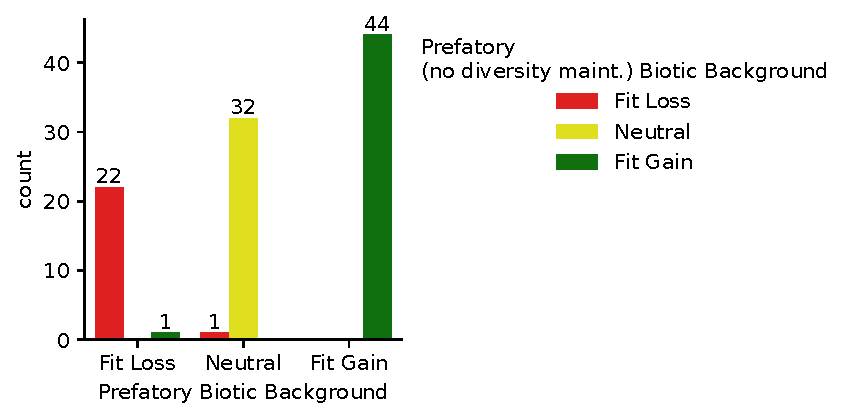
\includegraphics[width=\linewidth]{{submodule/dishtiny/binder/bucket=prq49/a=adaptation_assays+endeavor=16/teeplots/assay-subject=Specimen+hue=prefatory-no-diversity-maint-biotic-background+kind=count+viz=barlabel-catplot+x=prefatory-biotic-background+ext=}}
\caption{prefatory biotic background outcomes with and without diversity maintenance}
\end{subfigure}%
\hfill%
\begin{subfigure}[t]{0.49\textwidth}
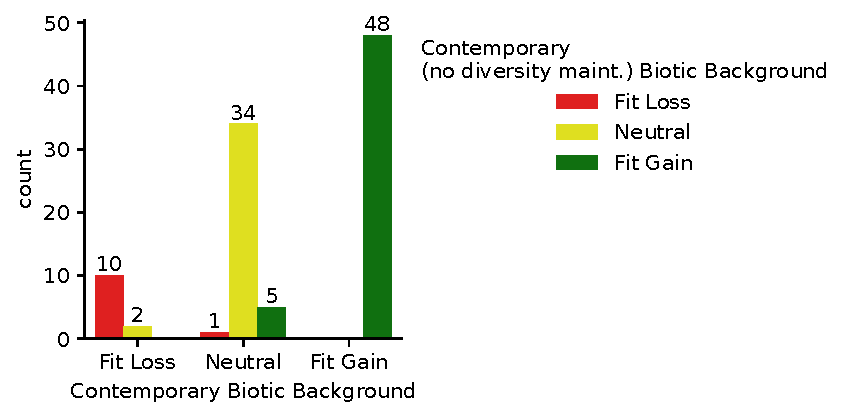
\includegraphics[width=\linewidth]{{submodule/dishtiny/binder/bucket=prq49/a=adaptation_assays+endeavor=16/teeplots/assay-subject=Specimen+hue=contemporary-no-diversity-maint-biotic-background+kind=count+viz=barlabel-catplot+x=contemporary-biotic-background+ext=}}
\caption{contemporary biotic background outcomes with and without diversity maintenance}
\end{subfigure}

\caption{
\textbf{Effect of diversity maintenance on adaptation assays with biotic background.}
\footnotesize
Joint distribution of competition experiments performed under biotic background conditions with diversity maintenance enabled and disabled.
Color coding denotes outcome without diversity maintenance and $x$ position denotes outcome with diversity maintenance.
Note that both plots above show distributions for adaptation assays on representative specimens.
Competition experiments without diversity maintenance were not performed for population-level adaptation.
See Figure \ref{fig:adaptation_assay_cartoon} for explanation of competition biotic backgrounds.
}
\label{fig:with_vs_without_diversity_maintenance}
\end{figure*}


To better characterize the mechanism behind fitness effects caused by the background strain, we performed additional specimen adaptation assays under biotic background conditions with diversity maintenance disabled.
This analysis allowed us to test whether action of the diversity maintenance mechanism, rather than direct interactions between the focal and background strains, caused the observed fitness effects.
Figure \ref{fig:with_vs_without_diversity_maintenance} compares adaptation assay outcomes with and without diversity maintenance under both the prefatory and contemporary biotic background conditions.
Outcomes were generally similar, and we observed only one sign-change difference: one specimen outcome was beneficial under prefatory biotic background conditions without diversity maintenance, but deleterious with diversity maintenance.
Further, without diversity maintenance, we still observed four outcomes that were advantageous under biotic conditions but deleterious under abiotic conditions (Figure \ref{fig:outcome_count_joint_distns:specimen_no_dm}).
So, biotic selective effects cannot be explained as an artifact of the diversity maintenance scheme.%
\footnote{
We also conducted specimen adaptation assays with diversity maintenance disabled under the control focal strain biotic background.
In these experiments, we again found no evidence for impact from the diversity maintenance scheme on results
(Supplementary Figure \ref{fig:baseline_fitness_gain_or_loss}).
}

\begin{sidewaysfigure*}
\thisfloatpagestyle{mylandscape}%
\rotatesidewayslabel%
\centering
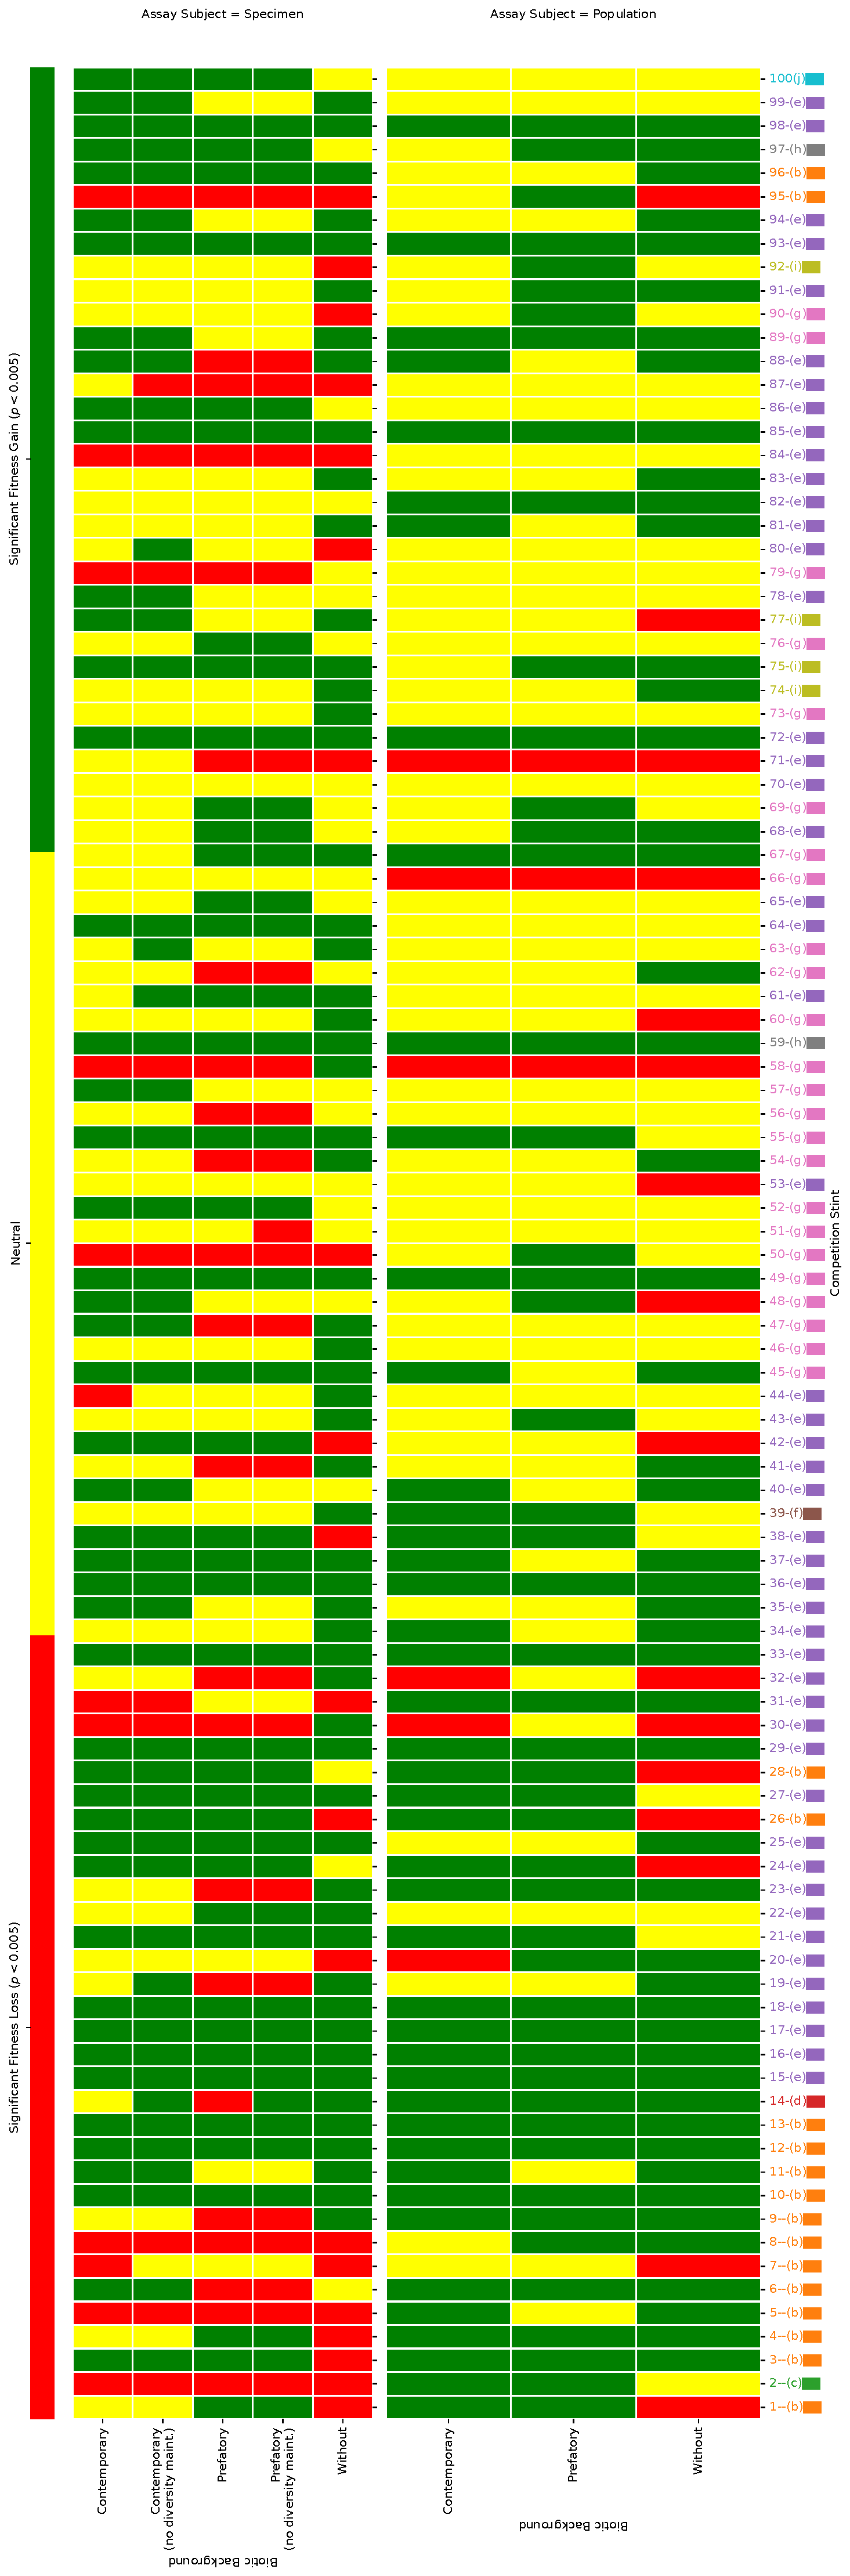
\includegraphics[width=\linewidth]{{submodule/dishtiny/binder/bucket=prq49/a=adaptation_assays+endeavor=16/teeplots/hue=fitness-gain-or-loss+viz=facet-heatmap+x=biotic-background+y=competition-stint+ext=}}

\caption{
\textbf{Adaptation Assay Outcomes.}
\footnotesize
Summary of adaptation assay outcomes for sampled representative specimen (top) and population-level adaptation (bottom).
Color coding and parentheticals of stint labels correspond to qualitative morph codes described in Table \ref{tab:morph_descriptions}.
See Figure \ref{fig:adaptation_assay_cartoon} for explanation of competition biotic backgrounds.
}
\label{fig:fitness_gain_or_loss}
\end{sidewaysfigure*}


Significant increases in fitness occur throughout the evolutionary history of the case study, but not at every stint.
Figure \ref{fig:fitness_gain_or_loss} summarizes the outcome of all adaptation assays stint-by-stint across evolutionary history.
Neutral outcomes appear to occur more frequently at later stints.
This may be indicative of slower evolutionary innovation, but may also result to some extent from simulation of fewer generations during evolutionary stints (Supplementary Figure \ref{fig:simulation}) and during competition experiments (Supplementary Figure \ref{fig:num_updates_elapsed_barplot}) due to slower execution of later genomes.

\begin{sidewaysfigure*}
\centering
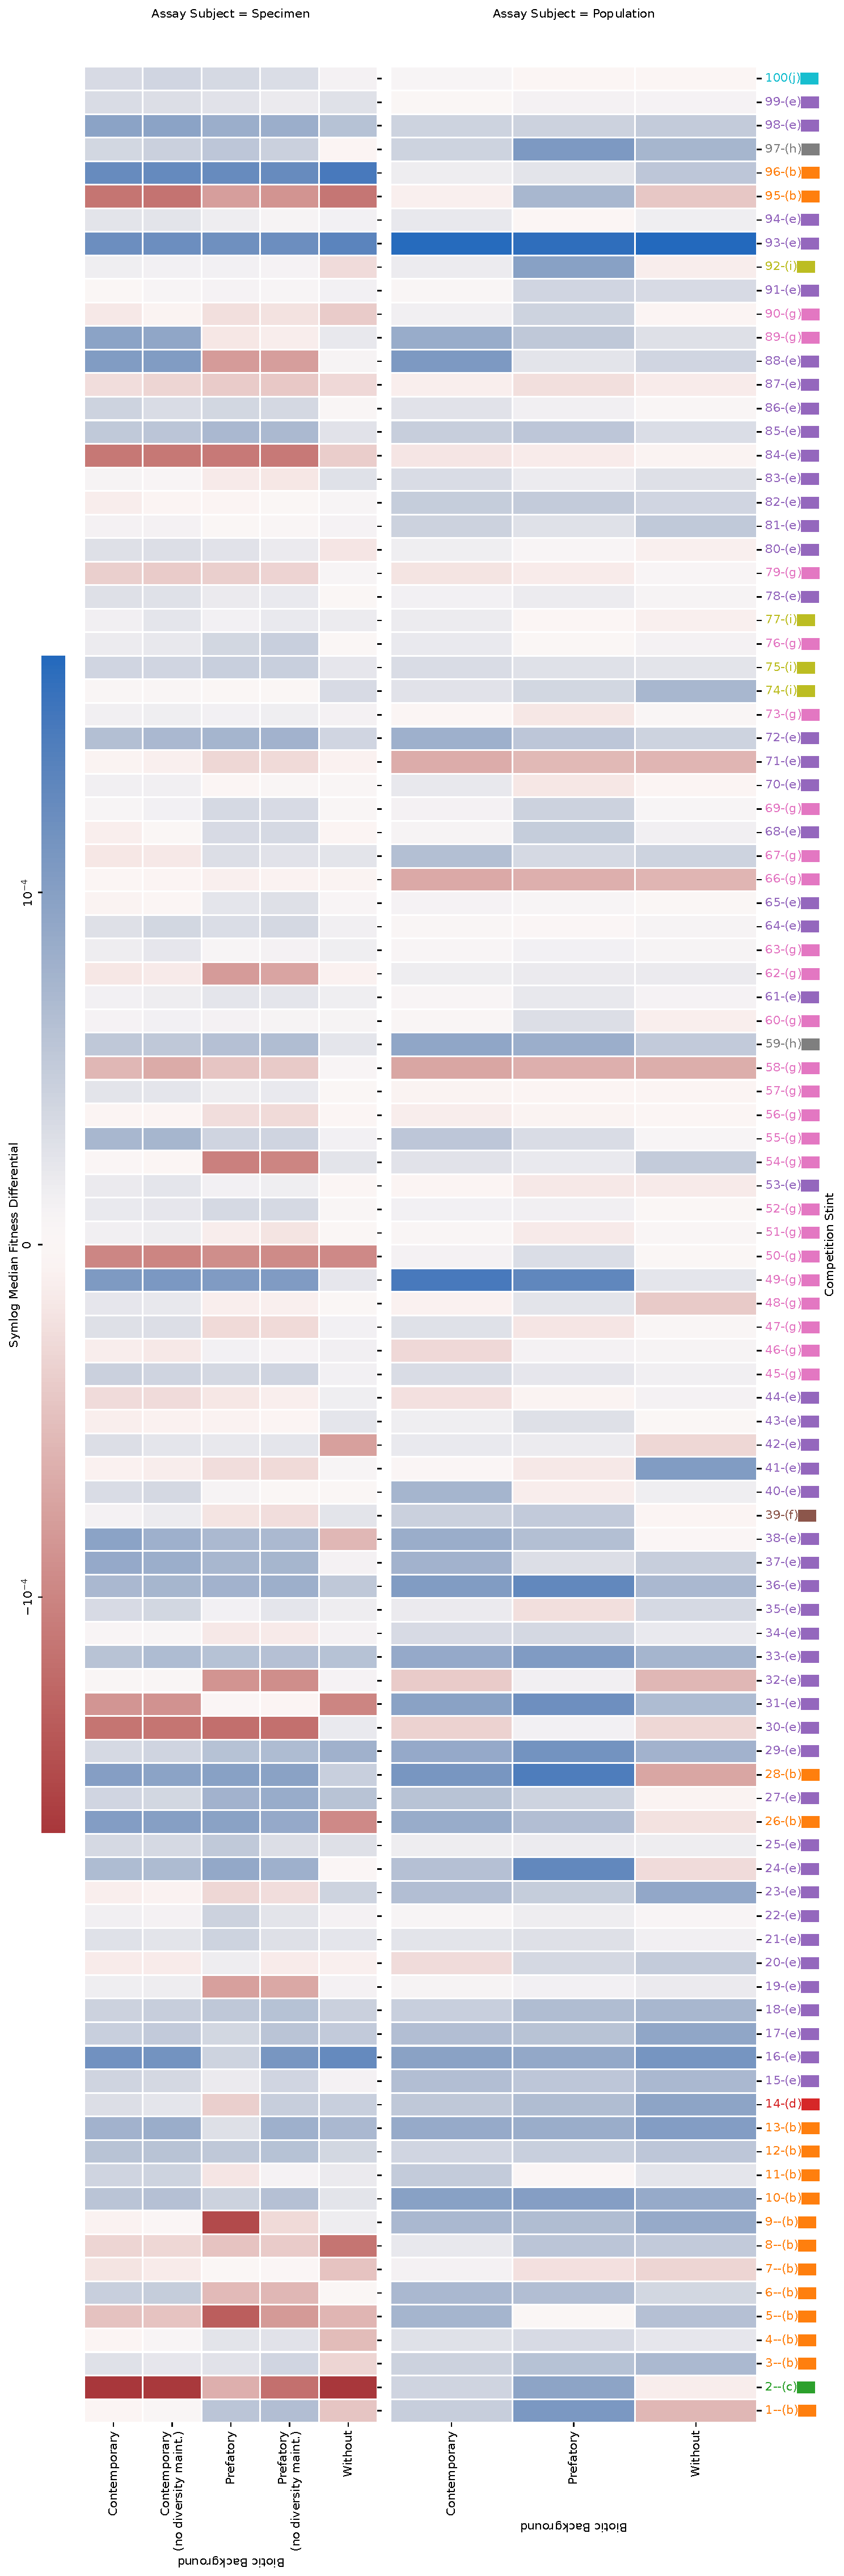
\includegraphics[width=\linewidth]{{submodule/dishtiny/binder/bucket=prq49/a=adaptation_assays+endeavor=16/teeplots/hue=symlog-median-fitness-differential+viz=facet-heatmap+x=biotic-background+y=competition-stint+ext=}}

\caption{
TODO
}
\label{fig:median_fitness_differential_symlog}
\end{sidewaysfigure*}


Figure \ref{fig:median_fitness_differential_symlog} shows the magnitudes of calculated fitness differentials for all adaptation assays.
Fitness differentials during the first 40 stints are generally higher magnitude than later fitness differentials, although a strong fitness differential occurs at stint 93.
Although the emergence of morphology $d$ was associated with significant increases in fitness in some specimen assays and morphologies $e$ and $g$ were associated with significant increases in fitness across all specimen assays (Figure \ref{fig:fitness_gain_or_loss}), the magnitude of these fitness differentials appears ordinary compared to fitness differentials at other stints (Figure \ref{fig:median_fitness_differential_symlog}).
Supplementary Figure \ref{fig:mean_competition_prevalence} shows mean end-competition prevalence across assays, telling a similar story.

\begin{figure}

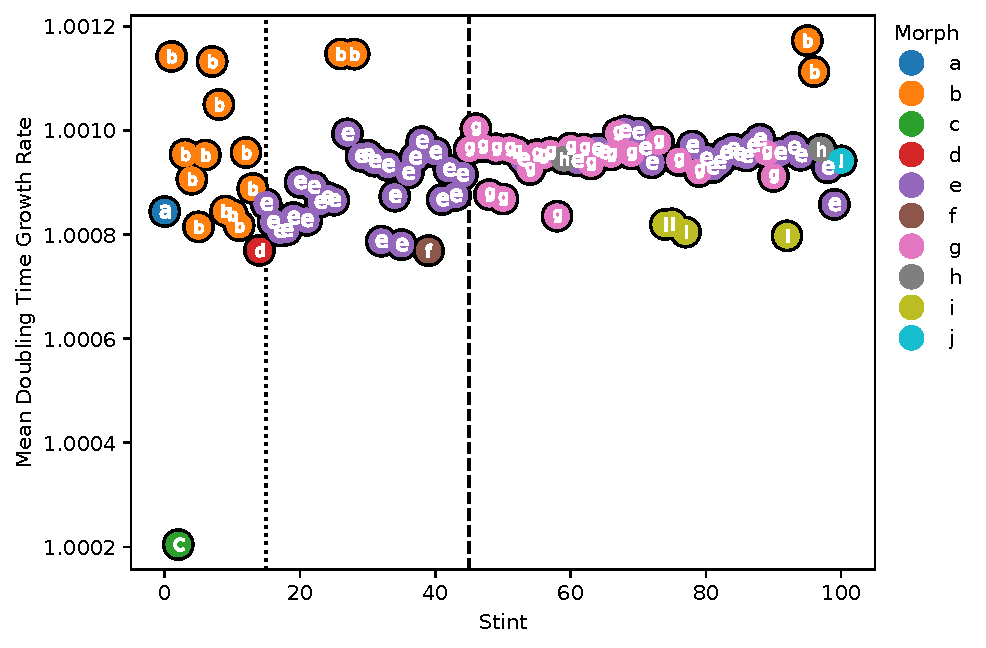
\includegraphics[width=\linewidth]{{plots/fitness/bucket=prq49+cat=morph+endeavor=16+transform=filter-Series-16005+viz=letterscatter-vline+x=stint+y=mean-doubling-time-growth-rate+ext=}}

\caption{Growth rate estimated from doubling time experiments, measuring time for a monoculture to grow from 0.25 maximum population size to 0.5 maximum population size.}
\label{fig:doubling_time}

\end{figure}


In addition to competition assays, we also measured growth rate of specimen strains by tracking doubling time (in updates) when seeded into quarter-full toroidal grids (Figure \ref{fig:doubling_time}).
Morph $b$ exhibited a fast growth rate early on that was never matched by later morphs.
This measure appears to be a poor overall proxy for fitness, highlighting the importance of biotic aspects of the simulation environment, which are not present in the empty space the assayed cells double into.


\subsection{Fitness Complexity}

\begin{figure}
\centering
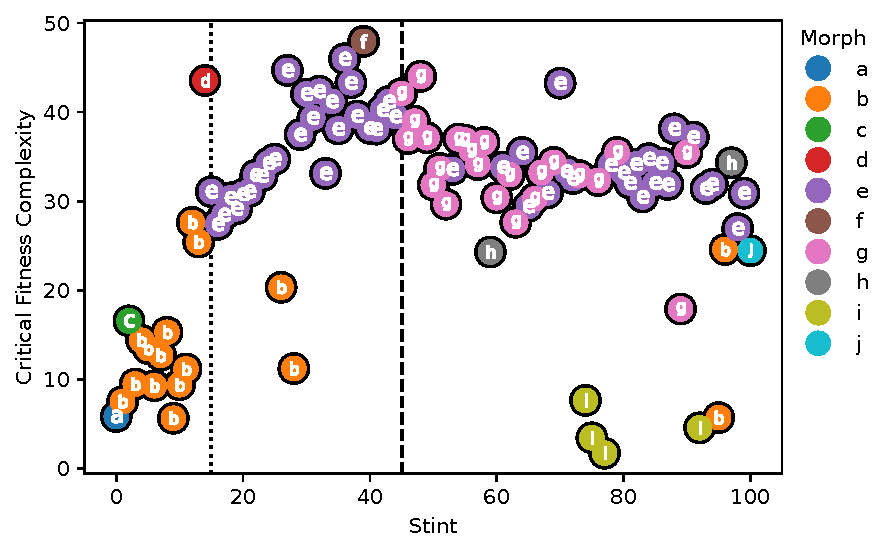
\includegraphics[width=0.5\textwidth]{{plots/critical_fitness_complexity/bucket=prq49+cat=morph+endeavor=16+transform=filter-Series-16005+viz=letterscatter-vline+x=stint+y=critical-fitness-complexity+ext=}}

\caption{
\textbf{Critical fitness complexity.}
\footnotesize
Number of single-site nopouts that significantly decrease fitness, adjusted for expected false positives.
Color coding and letters correspond to qualitative morph codes described in Table \ref{tab:morph_descriptions}.
Dotted vertical line denotes emergence of morph $e$.
Dashed vertical line denotes emergence of morph $g$.
}
\label{fig:critical_fitness_complexity}

\end{figure}%


Figure \ref{fig:critical_fitness_complexity} plots critical fitness complexity of specimens drawn from across the case study's evolutionary history.

Critical fitness complexity reaches more than 20 under morph $b$, jumps to more than 40 under morph $d$, and drops to slightly more than 30 for morph $e$.
Critical fitness complexity reaches a peak of 48 sites around stint 39, then levels out and decreases.
This decrease may in part be due to declining sensitivity of competition experiments due to slower simulation resulting in execution of fewer updates within the fixed-duration jobs (Supplementary Figure \ref{fig:num_updates_elapsed_heatmap}).

Phylogenetic analysis (Figure \ref{fig:phylo_parsimony_tree}) suggests independent origins of the critical fitness complexity in morph $d$ and morph $e$ --- the morph $d$ specimen from stint 14 is more closely related to the morph $b$ specimen from stint 13 than to the morph $e$ specimen from stint 15.
Likewise, specimens of lower complexity morphs $i$ and $b$ that appear past stint 70 appear to have independent evolutionary origins.

% The evolution of morph $g$ is not associated with a clear change in critical fitness complexity.

% Interpolated fitness complexity remains much more steady over the course of evolutionary history, although the certainty of our estimate of interpolated fitness complexity varies greatly.
% Figure \ref{fig:fitness_complexity:interpolated_fitness_complexity} shows this.
% Sometimes we were not able to estimate composite fitness complexity because the phenotype neutral nopout was not truly neutral --- it was significantly less fit than wildtype.

% Figure \ref{fig:fitness_complexity:composite_fitness_complexity} shows composite fitness complexity, the sum of interpolated fitness complexity and critical fitness complexity.
% The highest best estimate of composite fitness complexity was 64 sites at stint 61.
% The highest lower bound estimate of composite fitness complexity was 49 sites at stint 70.

\subsection{Interface Complexity}

% \pragmaonce

% adapted from https://www.overleaf.com/learn/latex/Commands
\providecommand{\dissertationonly}[1]{%
% adapted from https://tex.stackexchange.com/a/33577
\ifdefined\DISSERTATION%
#1%
\else%
\fi
}

\begin{figure*}
\dissertationonly{\captionsetup[subfigure]{font=scriptsize}}
\dissertationonly{\captionsetup{font=footnotesize}}
\begin{subfigure}[t]{0.49\textwidth}

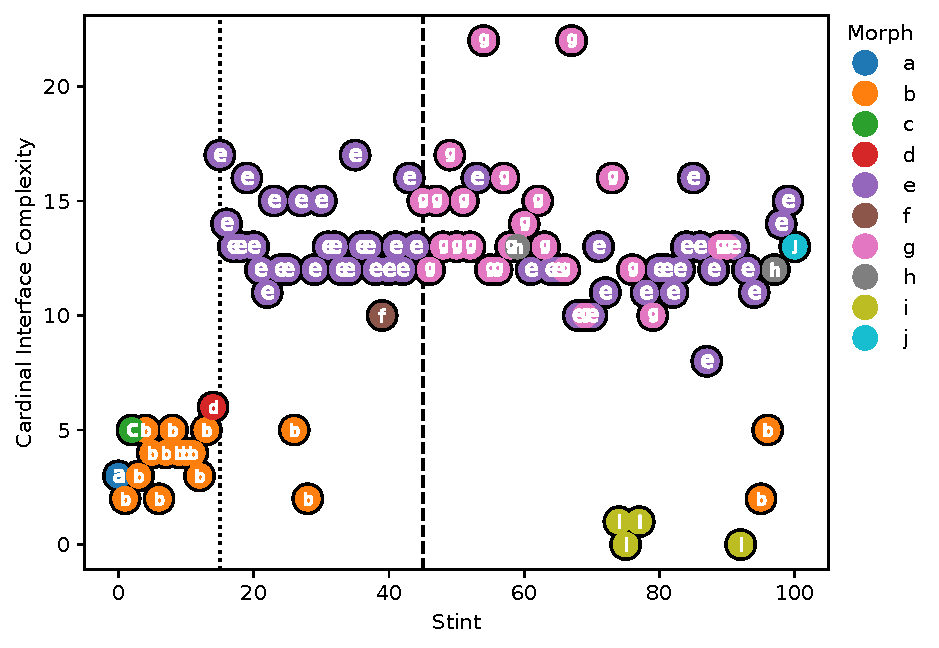
\includegraphics[width=\linewidth]{{plots/cardinal_interface_complexity/bucket=prq49+cat=morph+endeavor=16+transform=filter-Series-16005+viz=letterscatter+x=stint+y=cardinal-interface-complexity+ext=}}

\caption{Cardinal processor interface complexity, the total number of distinct interactions between a virtual CPU controlling cell behavior and its surroundings that contribute to fitness.
(Sum of Figures \labelcref{fig:interface_complexity:extrospective_interface_complexity,fig:interface_complexity:introspective_interface_complexity,fig:interface_complexity:writable_interface_complexity,fig:interface_complexity:intermessage_interface_complexity,fig:interface_complexity:intramessage_interface_complexity}.)}
\label{fig:interface_complexity:cardinal_interface_complexity}

\end{subfigure}%

\begin{subfigure}[t]{0.49\textwidth}

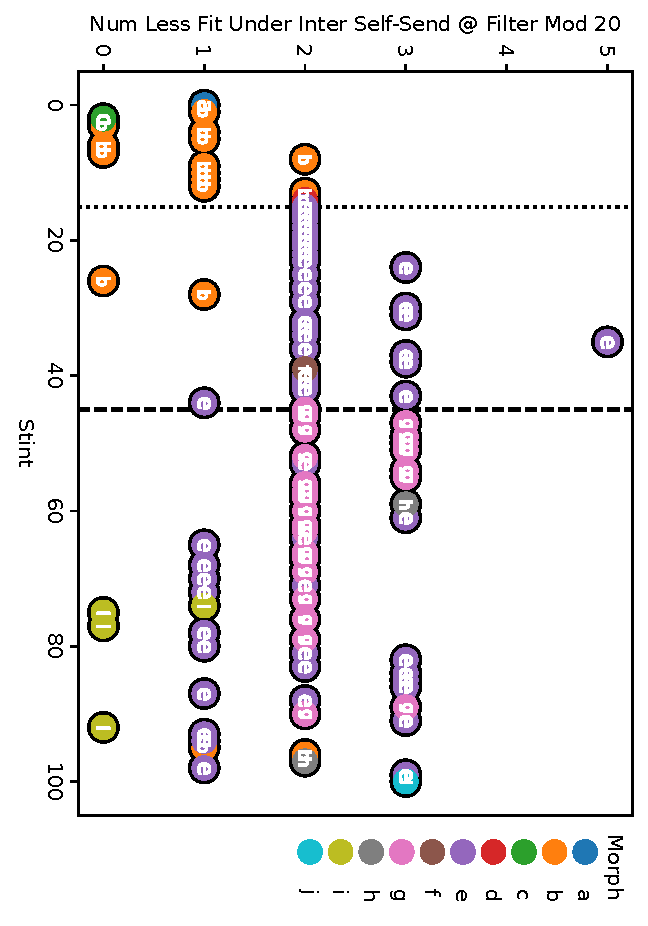
\includegraphics[width=\linewidth]{{plots/intermessage_interface_complexity/bucket=prq49+cat=morph+endeavor=16+transform=filter-Series-16005+viz=letterscatter-vline+x=stint+y=num-less-fit-under-inter-self-send-filter-mod-20+ext=}}

\caption{Intermessage interface complexity, the number of distinct inter-cell messages that contribute to fitness.}
\label{fig:interface_complexity:intermessage_interface_complexity}

\end{subfigure}%

\begin{subfigure}{0.5\textwidth}

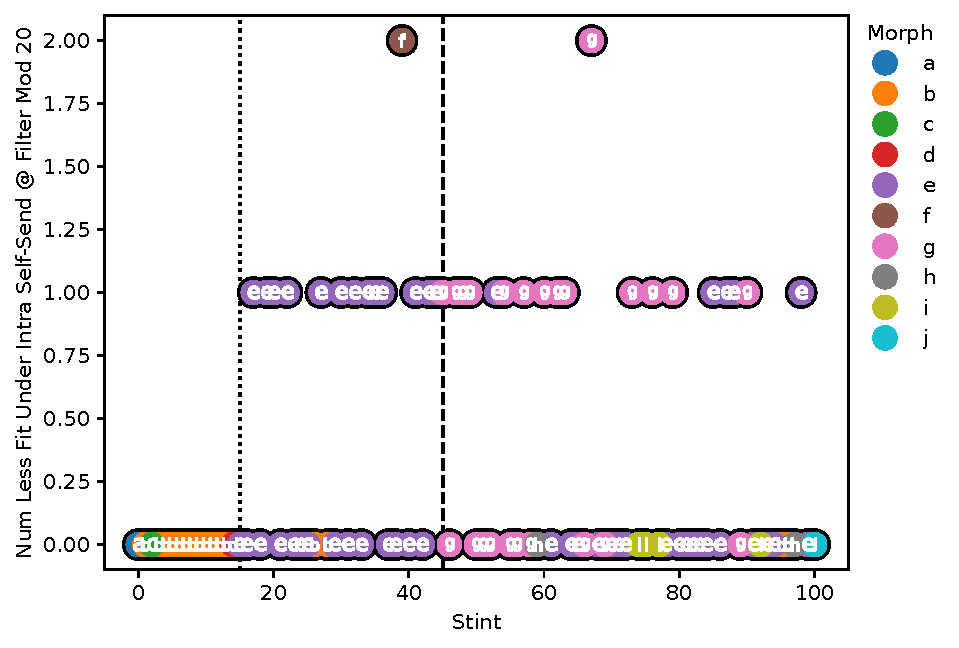
\includegraphics[width=\linewidth]{{plots/intramessage_interface_complexity/bucket=prq49+cat=morph+endeavor=16+transform=filter-Series-16005+viz=letterscatter-vline+x=stint+y=num-less-fit-under-intra-self-send-filter-mod-20+ext=}}

\caption{Intramessage interface complexity, the number of distinct inter-cell messages that contribute to fitness.}
\label{fig:interface_complexity:intramessage_interface_complexity}

\end{subfigure}%
\begin{subfigure}[t]{0.49\textwidth}

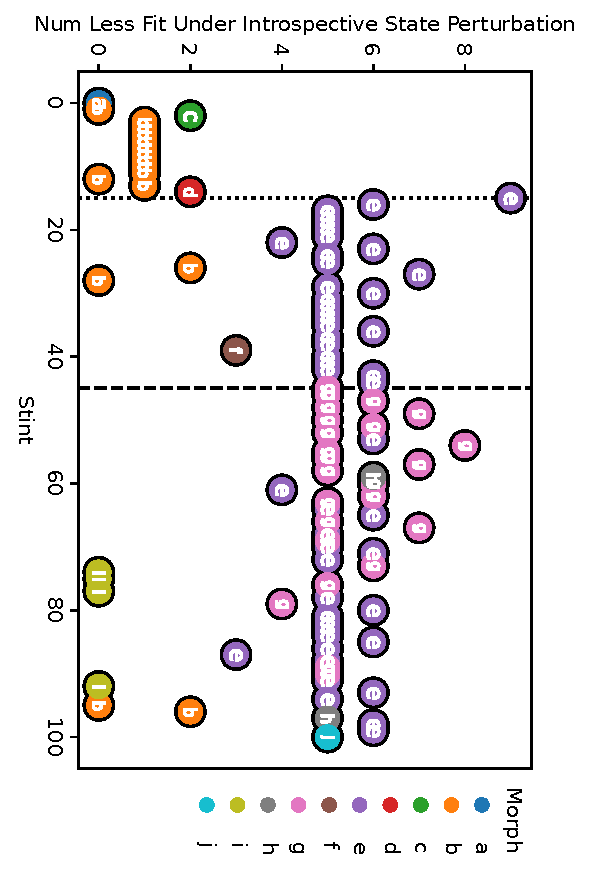
\includegraphics[width=\linewidth]{{plots/introspective_interface_complexity/bucket=prq49+cat=morph+endeavor=16+transform=filter-Series-16005+viz=letterscatter-vline+x=stint+y=num-less-fit-under-introspective-state-perturbation+ext=}}

\caption{Introspective interface complexity, the number of states viewed in the own cell that contribute to fitness. See Supplementary Figure \ref{fig:introspective_perturbation} for detail on the introspective states that contribute to fitness.}
\label{fig:interface_complexity:introspective_interface_complexity}

\end{subfigure}%

\begin{subfigure}{0.5\textwidth}

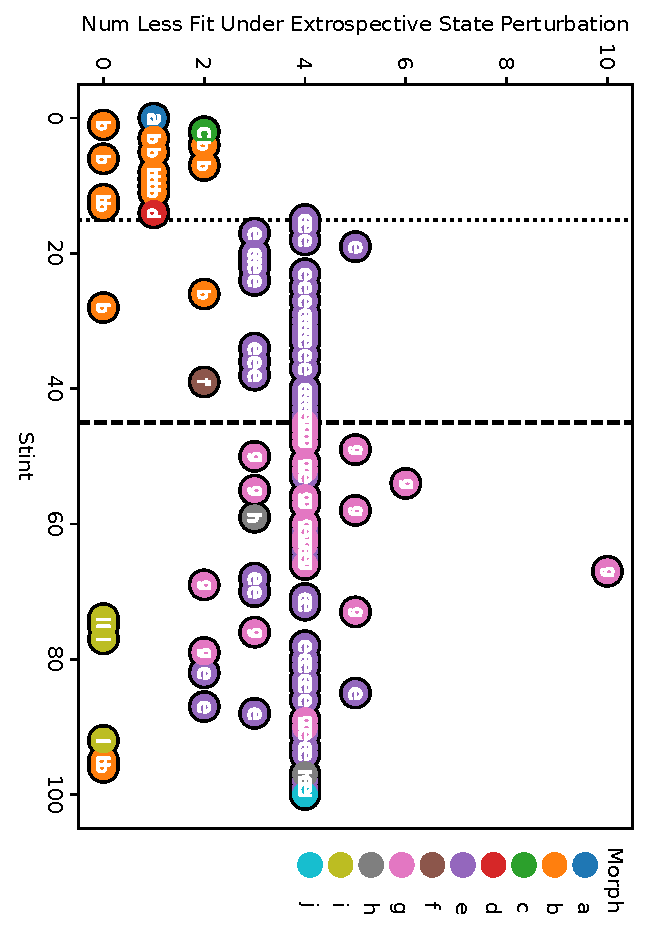
\includegraphics[width=\linewidth]{{plots/extrospective_interface_complexity/bucket=prq49+cat=morph+endeavor=16+transform=filter-Series-16005+viz=letterscatter-vline+x=stint+y=num-less-fit-under-extrospective-state-perturbation+ext=}}

\caption{ Extrospective interface complexity, the number of states viewed in neighboring cells that contribute to fitness.
See Supplementary Figure \ref{fig:extrospective_perturbation} for detail on the extrospective states that contribute to fitness. 
}
\label{fig:interface_complexity:extrospective_interface_complexity}

\end{subfigure}%
\begin{subfigure}{0.5\textwidth}

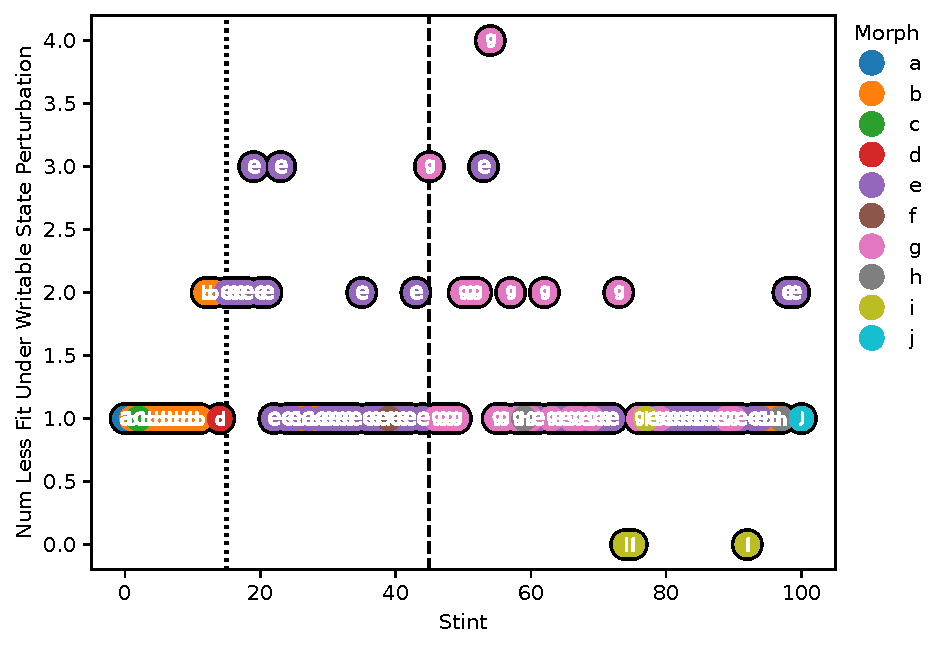
\includegraphics[width=\linewidth]{{plots/writable_interface_complexity/bucket=prq49+cat=morph+endeavor=16+transform=filter-Series-16005+viz=letterscatter-vline+x=stint+y=num-less-fit-under-writable-state-perturbation+ext=}}

\caption{Writable state interface complexity, the number of output states that contribute to fitness. See Supplementary Figure \ref{fig:writable_perturbation} for detail on the writable states that contribute to fitness.}
\label{fig:interface_complexity:writable_interface_complexity}

\end{subfigure}%

\caption{ Interface complexity estimates. Color coding and letters correspond to qualitative morph codes described in Table \ref{tab:morph_descriptions}.
Dotted vertical line denotes emergence of morph $e$.
Dashed vertical line denotes emergence of morph $g$.}
\label{fig:interface_complexity}
\end{figure*}


Figure \ref{fig:interface_complexity} summarizes cardinal processor interface complexity, as well as its constituent components, for specimens drawn from across the case study's evolutionary history.

Notably, cardinal processor interface complexity more than doubles from 6 interactions to 17 interactions coincident with the emergence of morph $e$ (Figure \ref{fig:interface_complexity:cardinal_interface_complexity}).
This is due to simultaneous increases in extrospective state sensing (2 to 9 states; Figure \ref{fig:interface_complexity:extrospective_interface_complexity}), introspective state sensing (1 to 4 states; Figure \ref{fig:interface_complexity:introspective_interface_complexity}), and writable state usage (1 to 2 states; Figure \ref{fig:interface_complexity:writable_interface_complexity}).

The emergence of morph $g$ coincided with an increase in writable state interface complexity from 1 to 3, as shown in Figure \ref{fig:interface_complexity:writable_interface_complexity}.
However, morph $g$ was not associated with other changes in other aspects of cardinal processor interface complexity.
The greatest observed cardinal processor interface complexity was 22 interactions at stints 54 and 67.

\subsection{Genome Size}

\begin{figure}
\centering
\begin{subfigure}{0.49\textwidth}
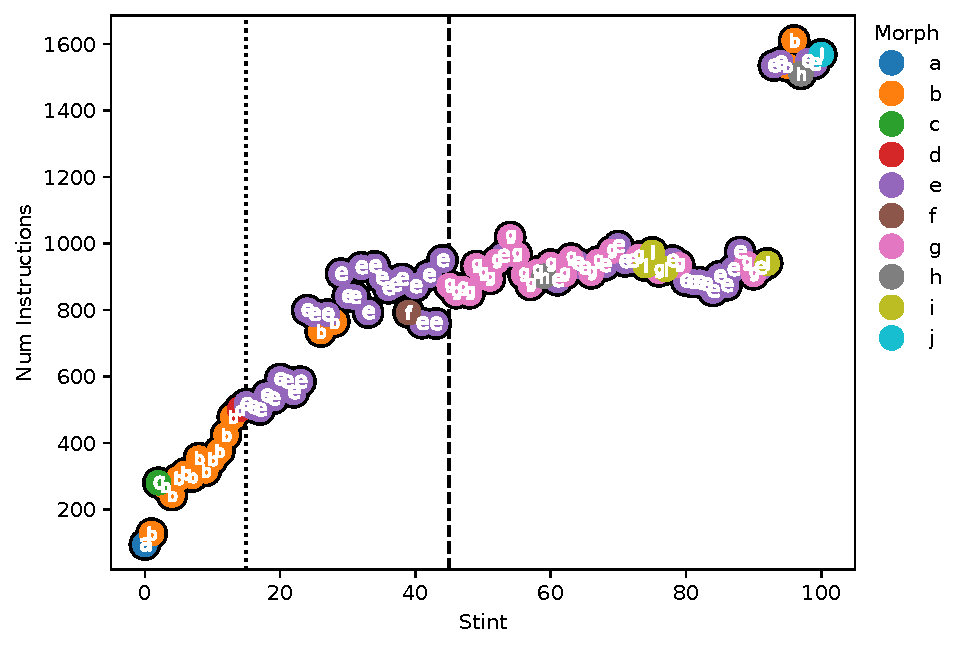
\includegraphics[width=\linewidth]{{submodule/dishtiny/binder/bucket=prq49/a=all_stints_all_series_profiles+endeavor=16/teeplots/bucket=prq49+cat=morph+endeavor=16+transform=filter-Series-16005+viz=letterscatter-vline+x=stint+y=num-instructions+ext=}}
\caption{instruction count}
\label{fig:instruction_count}
\end{subfigure}
\begin{subfigure}{0.49\textwidth}
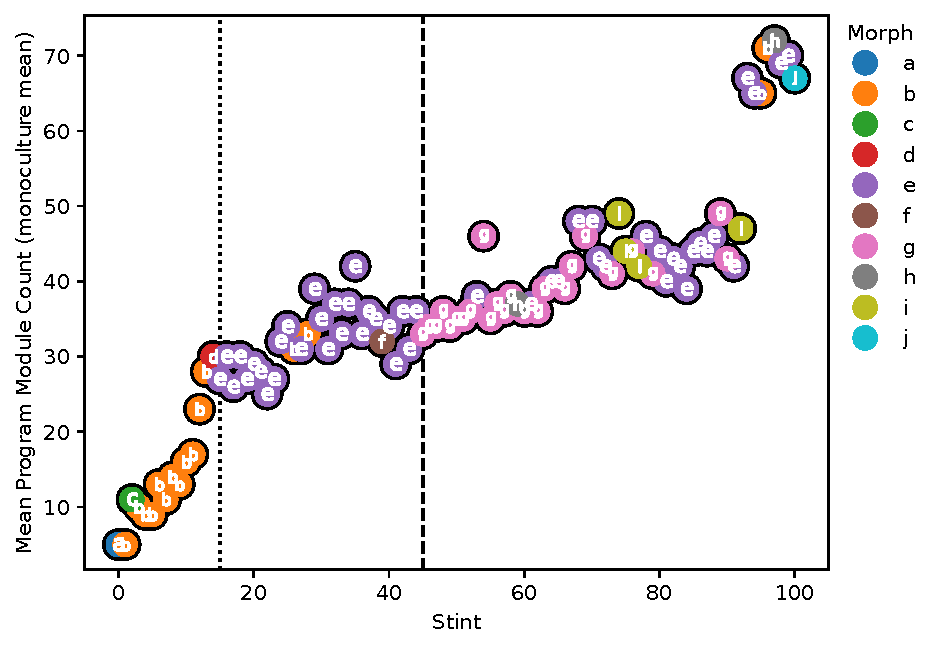
\includegraphics[width=\linewidth]{{submodule/dishtiny/binder/bucket=prq49/a=all_stints_all_series_profiles+endeavor=16/teeplots/bucket=prq49+cat=morph+endeavor=16+transform=filter-Series-16005+viz=letterscatter-vline+x=stint+y=mean-program-module-count-monoculture-mean+ext=}}
\caption{module count}
\label{fig:module_count}
\end{subfigure}
\begin{subfigure}{0.49\textwidth}
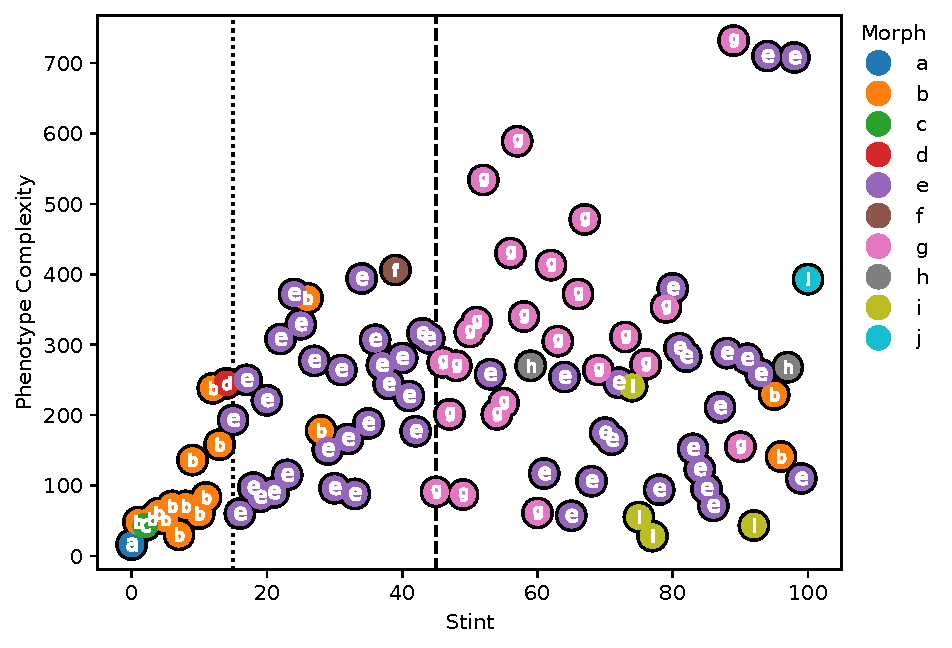
\includegraphics[width=\linewidth]{{plots/phenotype_complexity/bucket=prq49+cat=morph+endeavor=16+transform=filter-Series-16005+viz=letterscatter-vline+x=stint+y=phenotype-complexity+ext=}}
\caption{phenotype complexity}
\label{fig:phenotype_complexity}
\end{subfigure}

\caption{
Genome size of sampled focal strain specimens.
Instruction count is the total number of instructions present in the genome.
Module count is the number of tagged linear GP modules available for activation by signals from the environment, from other agents, or from within an agent.
Phenotype complexity is the number of genome sites that contribute to phenotype, measured as number sites remaining after phenotype-neutral nopout (Section \ref{sec:phenotype_neutral_nopout}).
This measure gives a sense of the number of ``active'' instructions that influence agents' behavior.
Color coding and letters correspond to qualitative morph codes described in Table \ref{tab:morph_descriptions}.
Dotted vertical line denotes emergence of morph $e$.
Dashed vertical line denotes emergence of morph $g$.
}
\label{fig:genome_size}

\end{figure}


Figure \ref{fig:genome_size} shows evolutionary trajectories of three genome size metrics in sampled focal strain specimens.
Instruction count and module count increased from 100 and 5 to around 800 and 30, respectively, between stints 0 and 40.
Within this period at stint 24, instruction count jumped from around 600 to more than 800 and module count jumped by about 5.
This was coincident with detection in our adaptation assays of population-level sign-change mediation of adaptation by the background strain (Figure \ref{fig:fitness_gain_or_loss}).
In sampled specimen fitness assays at stint 24, we detected significant increases in fitness in the presence of the background strain but no significant change in fitness in its absence.

Between stints 40 and 90, module count gradually increased to around 40 while instruction count remained stable.
Then, at stint 93, instruction count jumped to around 1,500 and module count jumped to around 60.
This was coincident with the strong fitness differentials observed at stint 93 (Figure \ref{fig:median_fitness_differential_symlog}).

To better understand the functional effects of changes in genome size, we additionally measured the number of instructions that affected agent phenotype, shown as ``phenotype complexity'' in Figure \ref{fig:phenotype_complexity}.
This measure can be considered akin to a count of ``active'' sites.

Phenotype complexity varied greatly stint to stint.
The median value increased from nearly 0 to around 200 sites between stints 0 and 40.
Between stints 40 and 90, we observed phenotype complexity values ranging from less than 100 to more than 500.
Morph $g$ specimens appear to show particularly great variance in phenotype complexity.
The first observed morph $g$ specimen at stint 45 exhibited relatively low phenotype complexity of around 100 active sites.
The highest phenotype complexity values of around 700 were measured from three specimens of morphs $e$ and $g$ in the last ten stints.
